%%%%%%%%%%%%%%%%%%%%%%%% editor.tex %%%%%%%%%%%%%%%%%%%%%%%%%%%%%
%
% sample root file for the contributions of a "contributed volume"
%
% Use this file as a template for your own input.
%
%%%%%%%%%%%%%%%%%%%%%%%%%%%%% Springer %%%%%%%%%%%%%%%%%%%%%%%%%%


% RECOMMENDED %%%%%%%%%%%%%%%%%%%%%%%%%%%%%%%%%%%%%%%%%%%%%%%%%%%
\documentclass[graybox, envcountchap, twocolum]{styles/svmult}

% general metadata:
\author{Author: idf@github}
\title{Algorithm Quicksheet}
\subtitle{Classical equations, diagrams and tricks in algorithm}
% choose options for [] as required from the list
% in the Reference Guide

\usepackage{amssymb,amsmath,bm}
\DeclareMathAlphabet{\mathcal}{OMS}{cmsy}{m}{n}
\usepackage{textcomp}
\newcommand\abs[1]{\left\lvert#1\right\rvert}
\usepackage{longtable}
\usepackage{algorithm2e}
\usepackage{tocbibind}
\usepackage[toc]{multitoc}
\usepackage{commons/commons}
\usepackage{commons/code_style}
\usepackage{style/customized}
\usepackage{listings}
\lstset{columns=fullflexible, commentstyle=\rm, basicstyle=\footnotesize} % remove columns=fullflexible for monospace

\usepackage{titlesec}
\titlespacing*{\section}{0pt}{5\baselineskip}{\baselineskip}

\renewcommand{\bibname}{References}
\usepackage{mathptmx}        % selects Times Roman as basic font
\usepackage{helvet}          % selects Helvetica as sans-serif font
\usepackage{courier}         % selects Courier as typewriter font
%\usepackage{type1cm}        % activate if the above 3 fonts are
                             % not available on  your system

\usepackage{makeidx}         % allows index generation
\usepackage{graphicx}        % standard LaTeX graphics tool
                             % when including figure files
\usepackage[justification=centering]{caption}
\usepackage{subfig}
\usepackage{multicol}        % used for the two-column index
\usepackage{multirow}
\usepackage[bottom]{footmisc}% places footnotes at page bottom
\usepackage[bookmarksnumbered=true,
            bookmarksopen=true,
            colorlinks=true,
            linkcolor=blue,
            anchorcolor=blue,
            citecolor=blue
           ]{hyperref}

\usepackage{comment}
%\excludecomment{figure}
\graphicspath{{figures/}}
\newcommand\AND{\ \&\ }
\newcommand\OR{\ |\ }
\newcommand\XOR{\wedge}
\newcommand\NOT{\ensuremath{\mathord{\sim}}}
\newcommand\SHIFTL{\ll}
\newcommand\SHIFTR{\gg}
% see the list of further useful packages in the Reference Guide

\makeindex             % used for the subject index
                       % please use the style svind.ist with
                       % your makeindex program

%%%%%%%%%%%%%%%%%%%%%%%%%%%%%%%%%%%%%%%%%%%%%%%%%%%%%%%%%%%%%%%%%
\usepackage[normalem]{ulem}

\begin{document}

\frontmatter%%%%%%%%%%%%%%%%%%%%%%%%%%%%%%%%%%%%%%%%%%%%%%%%%%%%%%

\onecolumn
\begin{titlepage}
\small{\urld{github.com/algorhythms/Algo-Quicksheet}}\\
\end{titlepage}

\newpage
\noindent \textcopyright  2015 github.com/idf \\
Except where otherwise noted, this document is licensed under a BSD 3.0
license (\urld{opensource.org/licenses/BSD-3-Clause}).

%%%%%%%%%%%%%%%%%%%%%%% dedic.tex %%%%%%%%%%%%%%%%%%%%%%%%%%
%
% sample dedication
%
% Use this file as a template for your own input.
%
%%%%%%%%%%%%%%%%%%%%%%%% Springer %%%%%%%%%%%%%%%%%%%%%%%%%%

\begin{dedication}
This book is dedicated to all Software Engineers.
\end{dedication}




%%%%%%%%%%%%%%%%%%%%%%%foreword.tex%%%%%%%%%%%%%%%%%%%%%%%%%%%
% sample foreword
%
% Use this file as a template for your own input.
%
%%%%%%%%%%%%%%%%%%%%%%%% Springer %%%%%%%%%%%%%%%%%%%%%%%%%%

\foreword

Use the template \textit{foreword.tex} together with the Springer document class SVMono (monograph-type books) or SVMult (edited books) to style your foreword\index{foreword} in the Springer layout. 

The foreword covers introductory remarks preceding the text of a book that are written by a \textit{person other than the author or editor} of the book. If applicable, the foreword precedes the preface which is written by the author or editor of the book.


\vspace{\baselineskip}
\begin{flushright}\noindent
Place, month year\hfill {\it Firstname  Surname}\\
\end{flushright}



%%%%%%%%%%%%%%%%%%%%%%preface.tex%%%%%%%%%%%%%%%%%%%%%%%%%%%%%%%%%%%%%%%%%
% sample preface
%
% Use this file as a template for your own input.
%
%%%%%%%%%%%%%%%%%%%%%%%% Springer %%%%%%%%%%%%%%%%%%%%%%%%%%

\preface
\section*{Introduction}
This quicksheet contains many classical equations and diagrams for algorithm, which helps you quickly recall knowledge and ideas in algorithm.\\

This quicksheet has three significant advantages:
\begin{enumerate}
\item Non-essential knowledge points omitted
\item Compact knowledge representation
\item Quick recall
\end{enumerate}
\section*{How to Use This Quicksheet}
You should not attempt to remember the details of an algorithm. Instead, you should know:
\begin{enumerate}
\item What problems this algorithm solves.
\item The benefits of using this algorithm compared to others.
\item The important clues of this algorithm so that you can derive the details of the algorithm from them.
\end{enumerate}
Only dives into the code when you is unable to reconstruct the algorithm from the hits and the important clues. 

\vspace{\baselineskip}
\begin{flushright}\noindent
At GitHub, June 2015\hfill {\it github.com/idf} \\
\end{flushright}

%%%%%%%%%%%%%%%%%%%%%%%acknow.tex%%%%%%%%%%%%%%%%%%%%%%%%%%%%%%%%%%%%%%%%%
% sample acknowledgement chapter
%
% Use this file as a template for your own input.
%
%%%%%%%%%%%%%%%%%%%%%%%% Springer %%%%%%%%%%%%%%%%%%%%%%%%%%

\extrachap{Acknowledgements}

Use the template \emph{acknow.tex} together with the Springer document class SVMono (monograph-type books) or SVMult (edited books) if you prefer to set your acknowledgement section as a separate chapter instead of including it as last part of your preface.



\tableofcontents
%%%%%%%%%%%%%%%%%%%%clist.tex %%%%%%%%%%%%%%%%%%%%%%%%
%                                                    
% sample list of contributors and their addresses    
%                                                    
% Use this file as a template for your own input.    
%                                                    
%%%%%%%%%%%%%%%%%%%%%%%% Springer %%%%%%%%%%%%%%%%%%%%
\contributors

\begin{thecontriblist}
Daniel D. Zhang (\urld{github.com/idf})
\end{thecontriblist}

%%%%%%%%%%%%%%%%%%%%%%%acronym.tex%%%%%%%%%%%%%%%%%%%%%%%%%%%%%%%%%%%%%%%%%
% sample list of acronyms
%
% Use this file as a template for your own input.
%
%%%%%%%%%%%%%%%%%%%%%%%% Springer %%%%%%%%%%%%%%%%%%%%%%%%%%

\Extrachap{Abbreviations}

\runinhead{A} Array 
\runinhead{idx} Index
\runinhead{TLE} Time Limit Exceeded
\runinhead{MLE} Memory Limit Exceeded
\runinhead{dp} Dynamic programming 
\runinhead{def} Definition
\runinhead{ptr} Pointer 
\runinhead{len} Length
\runinhead{asc} Ascending
\runinhead{desc} Descending
\runinhead{pred} Predecessor
\runinhead{succ} Successor
\runinhead{$\pi$/pi} The parent of a child
\runinhead{bfs} Breadth-first search
\runinhead{dfs} Depth-first search 
\runinhead{mat} Matrix
\runinhead{ADT} Abstract Data Type
\runinhead{aka} Also known as

\Extrachap{Notations}\label{sec:Notation}

\section*{General Math Notations}

\begin{longtable}{cl}
\hline\noalign{\smallskip}
\textbf{Symbol} & \textbf{Meaning} \\
\noalign{\smallskip}\hline\noalign{\smallskip}
$\lfloor x \rfloor$ & Floor of $x$, i.e. round down to nearest integer\\
$\lceil x \rceil$ & Ceiling of $x$, i.e. round up to nearest integer\\
floor(key) & the largest key $\leq$ the given key \\
ceil(key) & the smallest key $\geq$ the given key \\
$\log x$ & The base of logarithm is 2 unless otherwise stated\\
$a \wedge b$ & Logical AND\\
$a \vee b$ & Logical OR\\
$\neg a $ & Logical NOT\\
$a\AND b$ & Bit AND\\
$a \OR b$ & Bit OR\\
$a \XOR  a$ & Bit XOR\\
$\NOT a$ & Bit NOT\\
$\SHIFTL a$ & Bit shift left\\
$\SHIFTR a$ & Bit shift right\\
$\infty$ & Infinity\\
$\rightarrow$ & Tends towards, e.g., $n \rightarrow \infty$\\
$\propto$ &Proportional to; $y = ax$ can be written as $y \propto x$\\
$\abs{x}$ & Absolute value\\
$||\vec{a}||$ & $L_2$ distance (Euclidean distance) of a vector; norm-2 \\
$\abs{\mathcal{S}}$ & Size (cardinality) of a set\\
$n!$ & Factorial function\\
$\triangleq$ & Defined as\\
$O(\cdot)$ & Big-O: roughly means order of magnitude\\
$\mathbb{R}$ & The real numbers\\
$0:n$ & Range (Python convention): $0:n = {0, 1, 2,...,n-1}$\\
$\approx$ & Approximately equal to\\
$\sim$ & Tilde, the leading term of mathematical expressions \\
$\arg\max\limits_x f(x)$ & Argmax: the value $x$ that maximizes $f$\\
$\binom{n}{k}$ & $n$ choose $k$ , equal to $\frac{n!}{k!(n-k)!}$\\
$range(i,j)$ & range of number from i (inclusive) to j (exclusive) \\
$A[i:j]$ & subarray consist of $A_i, A_{i+1}, ..., A_{j-1}$.
\noalign{\smallskip}\hline\noalign{\smallskip}
\end{longtable}


\twocolumn



\mainmatter%%%%%%%%%%%%%%%%%%%%%%%%%%%%%%%%%%%%%%%%%%%%%%%%%%%%%%%
%%%%%%%%%%%%%%%%%%%%%%part.tex%%%%%%%%%%%%%%%%%%%%%%%%%%%%%%%%%%
% 
% sample part title
%
% Use this file as a template for your own input.
%
%%%%%%%%%%%%%%%%%%%%%%%% Springer %%%%%%%%%%%%%%%%%%%%%%%%%%

\begin{partbacktext}
\part{Part Title}
\noindent Use the template \emph{part.tex} together with the Springer document class SVMono (monograph-type books) or SVMult (edited books) to style your part title page and, if desired, a short introductory text (maximum one page) on its verso page in the Springer layout.

\end{partbacktext}
% complexity
\chapter{Time Complexity}

\section{Basic Counts}
\rih{Double for-loops} 
$$
\sum_{i=1}^N{\sum_{j=i}^N{1}} = {N \choose 2} \sim \frac{1}{2} N^2
$$
$$
\sum_{i=1}^N{\sum_{j=i}^N{1}} \sim \int_{x=1}^N \int_{y=x}^N  \mathrm{d}y\, \mathrm{d}x
$$
\rih{Triple for-loops}
$$
\sum_{i=1}^N{\sum_{j=i}^N{\sum_{k=1}^N{1}}} = {N \choose 3} \sim \frac{1}{6} N^3
$$
$$
\sum_{i=1}^N{\sum_{j=i}^N{\sum_{k=1}^N{1}}} \sim \int_{x=1}^N \int_{y=x}^N \int_{z=y}^N \mathrm{d}z\,
\mathrm{d}y\, \mathrm{d}x
$$

\section{Solving Recurrence Equations}
Basic recurrence equation solving techniques:
\begin{enumerate}
\item Guessing and validation
\item Telescoping
\item Recursion tree
\item Master Theorem
\end{enumerate}

\subsection{Master Theorem}
Recurrence relations:
$$T(n) = a \; T\!\left(\frac{n}{b}\right) + f(n)\mbox{, where }a \geq 1 \mbox{, } b > 1$$

Notice that $b>1$ rather than $b\geq1$.

\subsubsection*{Case 1}
If:
$$f(n) = o(n^{\log_b a})$$

, where in the condition it is $o$ rather than $O$. \\\\
Then:
$$T(n) = \Theta(n^{\log_b a})$$
\subsubsection*{Case 2}
If:
$$f(n) = \Theta(n^{\log_b a} \log^{k} n)$$

, for some constant $k \geq 0$\\\\
Then:
$$
T(n) = \Theta(n^{\log_b a} \log^{k+1} n)
$$

, typically $k=0$ in most cases. 
\subsubsection*{Case 3}
If:
$$f(n) = \omega(n^{\log_b a})$$

, where in the condition it is $\omega$ rather than $\Omega$. \\\\
And with regularity condition:
$$f(\frac{n}{b}) \le k f(n)$$

, for some constant $k < 1$ and sufficiently large $n$\\\\
Then:
$$T\left(n \right) = \Theta\left(f(n) \right)$$
\section{Useful Math Equations}
Euler:
$$
\frac{1}{2}+\frac{1}{3}+\frac{1}{4} + ... + \frac{1}{n} = \ln{n}
$$
Logarithm power: 
$$
a^{\log_b^n} &= n^{\log_b^a}
$$

proof:
\begin{align*}
a^{\log_b^n} &= n^{\log_b^a} \\
\Leftarrow \ln{a^{\log_b^n}} &= \ln{n^{\log_b^a}}\\
\Leftarrow  \frac{\ln n}{\ln b}\ln a &=\frac{\ln a}{\ln b}\ln n
\end{align*}

\chapter{Memory Complexity}

\section{Introduction}
When discussing memory complexity, need to consider both 
\begin{enumerate}
\item \textbf{Heap}: the declared variables' size.
\item \textbf{Stack}: the recursive functions' call stack.
\end{enumerate}}
\subsection{Memory for Data Type}
The memory usage is based on Java.\\

\begin{tabular}{ll}
\hline\noalign{\smallskip}
\textbf{Type} & \textbf{Bytes} \\
\noalign{\smallskip}\hline\noalign{\smallskip}

boolean & 1 \\
byte & 1 \\
char & 2 \\
int & 4 \\
float & 4 \\
long & 8 \\
double & 8\\

\noalign{\smallskip}\hline\noalign{\smallskip}
\caption {for primitive types}
\end{tabular}

\begin{tabular}{ll}
\hline\noalign{\smallskip}
\textbf{Type} & \textbf{Bytes} \\
\noalign{\smallskip}\hline\noalign{\smallskip}

char[] & 2N+24 \\
int[] & 4N+24 \\
double[] & 8N+24 \\
T[] & 8N+24 \\

\noalign{\smallskip}\hline\noalign{\smallskip}
\caption{for one-dimensional arrays}
\end{tabular}

\begin{tabular}{ll}
\hline\noalign{\smallskip}
\textbf{Type} & \textbf{Bytes} \\
\noalign{\smallskip}\hline\noalign{\smallskip}

char[][] & 2MN \\
int[][] & 4MN \\
double[][] & 8MN \\

\noalign{\smallskip}\hline\noalign{\smallskip}
\caption{for two-dimensional arrays}
\end{tabular}

\begin{tabular}{ll}
\hline\noalign{\smallskip}
\textbf{Type} & \textbf{Bytes} \\
\noalign{\smallskip}\hline\noalign{\smallskip}

Object overhead & 16 \\
Reference & 8 \\
Padding & 8x \\

\noalign{\smallskip}\hline\noalign{\smallskip}
\caption{for objects}
\end{tabular}
\\
Notice:
\begin{enumerate}
\item The reference takes memory of 8 bytes. 
\item Reference includes object reference and innner class reference.
\item T[] only considers reference; if consider underlying data structure, the memory is 8N+24+xN, where $x$ is the underlying data structure memory for each element.
\item Padding is to make the object memory size of 8's multiple.
\end{enumerate}

\subsection{Example}
The generics is passed as Boolean:
\begin{java}
public class Box<T> {   // 16 (object overhead)
    private in N;       // 4 (int)
    private T[] items;  // 8 (reference to array)
                        // 8N+24 (array of Boolean references)
                        // 24N (underlying Boolean objects)
                        // 4 (padding to round up to a multiple)
}
\end{java} 

Notice the multiple levels of references. 


% data structure
\chapter{Basic Data  Structures}


\section{Introduction}
Abstract Data Types (ADT):
\begin{enumerate}
\item Queue
\item Stack
\item HashMap
\end{enumerate}
Implementation (for both queue and stack):
\begin{enumerate}
\item Linked List
\item Resizing Array:
\begin{enumerate}
\item Doubling: when full (100\%).
\item Halfing: when one-quarter full (100\%). 
\end{enumerate}}
\end{enumerate}}
Python Library:
\begin{enumerate}
\item \pythoninline{collections.deque} \footnote{The naming in Python collections is awkward: \href{http://stackoverflow.com/questions/18953681/naming-convention-in-collections-why-are-some-lowercase-and-others-capwords}{discussion}.}
\item \pythoninline{list}
\item \pythoninline{dict, OrderedDict, DefaultDict}
\end{enumerate}} 
Java Library:
\begin{enumerate}
\item \javainline{java.util.Stack<E>}
\item \javainline{java.util.LinkedList<E>}
\item \javainline{java.util.HashMap<K, V>; java.util.TreeMap<K, V>}
\end{enumerate}}

\section{Stack}
\subsection{Stack and Recursion}
How a compiler implements a function:
\begin{enumerate}
\item Function call: push local environment and return address
\item Return: pop return address and local environment. 
\end{enumerate}

Recursive function: function calls itself. It can always be implemented by using an explicit stack to remove recursion. 

\subsection{Usage}
The core philosophy of using stack is to maintain a relationship invariant among stack element. 

The \textbf{relationship invariants} can be:
\begin{enumerate}
\item strictly asc/ strictly desc
\item non-desc/ non-asc
\end{enumerate}

\subsection{Applications}
\runinhead{Largest Rectangle.} Find the largest rectangle in the matrix (histogram). Given $n$ non-negative integers representing the histogram's bar height where the width of each bar is 1, find the area of largest rectangle in the histogram. 

\begin{figure}[hbtp]
\centering
\subfloat{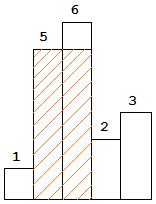
\includegraphics[scale=2.00]{histogram_area}}
\caption{Largest rectangle in histogram}
\label{fig:histogram_area}
\end{figure}

Keep a stack storing the bars in non-decreasing, then calculate the area by popping out the stack to get the currently lowest bar which determines the height of the rectangle.
\\
Core clues:
\begin{enumerate}
\item Maintain the non-decreasing stack. slow performance 
\item Popping triggers the calculation of area
\item Calculate the rectangle width by index diff
\item Post-processing in the end
\end{enumerate}
\newpage
Code:
\begin{python}
def largestRectangleArea(self, height):
    n = len(height)
    gmax = -sys.maxint-1
    stk = []  # store the idx, non-decreasing stack

    for i in xrange(n):
        while stk and height[stk[-1]] > height[i]:
            last = stk.pop()
            if stk:  # calculate area when popping
                area = height[last]*(i-(stk[-1]+1))
            else:
                area = height[last]*i
            gmax = max(gmax, area)

        stk.append(i)

    # after array scan, process the dangling stack
    i = n
    ...

    return gmax
\end{python}


\subsection{All nearest smaller values}\label{allNearestSmaller}
\textbf{Nearest smaller}. Left neighbor of a value $v$ to be the value that occurs prior to $v$, is smaller than $v$, and is closer in position to $v$ than any other smaller value.

For each position in a sequence of numbers, search among the \textit{previous} positions for the last position that contains a smaller value. 

Core clues:
\begin{enumerate}
\item Maintain a \textit{strictly increasing} stack.  
\item If all nearest \textit{larger} values, maintain a \textit{strictly decreasing} stack.  
\end{enumerate}

\begin{python}
def allNearestSmaller(self, A):
    P = [-1 for _ in A]
    stk = []
    for i, v in enumerate(A):
        while stk and A[stk[-1]] >= v: stk.pop()

        if stk:
            P[i] = stk[-1]
        else:
            P[i] = -1  # no preceding smaller value
            
        stk.append(i)  # store the idx or val

    return P
\end{python}

\section{Map}
\subsection{Math relations}
\textbf{1-1 Map}. Mathematically, full projection. One map, dual entries.
\begin{python}
class OneToOneMap(object):
    def __init__(self):
        self.m = {}  # keep a single map

    def set(self, a, b):
        self.m[a] = b
        self.m[b] = a

    def get(self, a):
        return self.m.get(a)
\end{python}
\subsection{Operations}
\runinhead{Sorting by value.} Sort the map entries by values \pyinline{itemgetter}.
\begin{python}
from operators import itemgetter 
sorted(hm.items(), key=itemgetter(1), reverse=True)
\end{python}

\chapter{Linked List}


\section{Operations}
\subsection{Fundamentals}
Get the $pre$ reference:
\begin{python}
dummy = Node(0)
dummy.next = head
pre = dummy
cur = pre.next
\end{python}

\subsection{Basic Operations}
\begin{enumerate}
\item Get the length
\item Get the $i$-th object
\item Delete a node 
\item Reverse
\begin{figure}[]
\centering
\subfloat{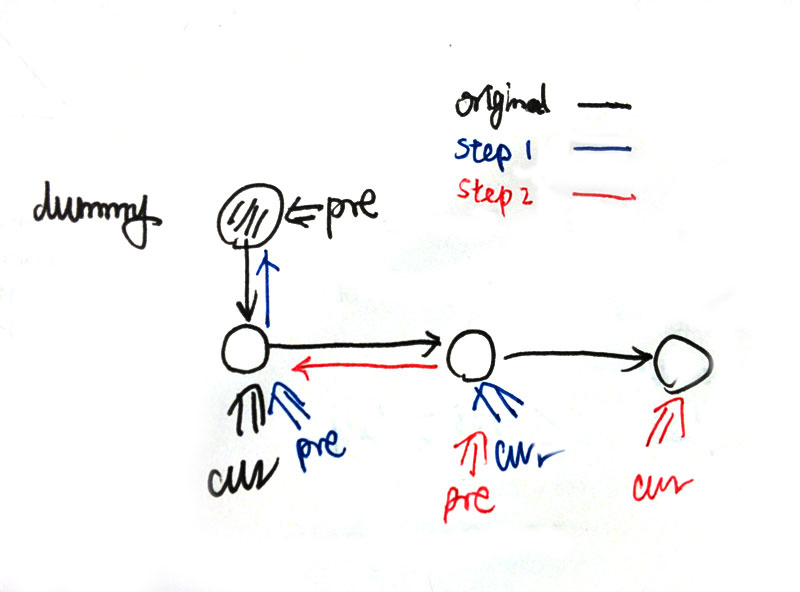
\includegraphics[scale=1.0]{ll_reverse}}
\caption{Reverse the linked list}
\label{fig:LABEL}
\end{figure}
\begin{python}
def reverseList(self, head):
    dummy = ListNode(0)
    dummy.next = head

    pre = dummy
    cur = pre.next
    while pre and cur:
        pre, cur.next, cur = cur, pre, cur.next
        # incorrect evaluation order:
        # pre, cur, cur.next = cur, cur.next, pre 

    dummy.next.next = None  # original head
    return pre  # new head
\end{python}
Notice: the evaluation order for the swapping the nodes and links. 
\end{enumerate}

\subsection{Combined Operations}
In $O(n)$ without extra space:
\begin{enumerate}
\item Determine whether two lists intersects
\item Determine whether the list is palindrome 
\item Determine whether the list is acyclic
\end{enumerate}

\section{Combinations}
\subsection{LRU}
Core clues:
\begin{enumerate}
\item Ensure $O(1)$ find $O(1)$ deletion. 
\item Doubly linked list + map.
\item Keep both \pyinline{head} and \pyinline{tail} pointer.
\item Operations on doubly linked list are case by case.  
\end{enumerate}
\begin{python}
class Node(object):
    def __init__(self, key, val):
        self.key = key
        self.val = val
        self.pre, self.next = None, None


class LRUCache(object):
    def __init__(self, capacity):
        self.cap = capacity
        self.map = {}  # key to node
        self.head = None
        self.tail = None

    def get(self, key):
        if key in self.map:
            cur = self.map[key]
            self._elevate(cur)
            return cur.val

        return -1

    def set(self, key, value):
        if key in self.map:
            cur = self.map[key]
            cur.val = value
            self._elevate(cur)
        else:
            cur = Node(key, value)
            self.map[key] = cur
            self._appendleft(cur)

            if len(self.map) > self.cap:
                last = self._pop()
                del self.map[last.key]

    # doubly linked-list operations only
    def _appendleft(self, cur):
        """Normal or initially empty"""
        if not self.head and not self.tail:
            self.head = cur
            self.tail = cur
            return

        head = self.head
        cur.next, cur.pre, head.pre = head, None, cur
        self.head = cur

    def _pop(self):
        """Normal or resulting empty"""
        last = self.tail
        if self.head == self.tail:
            self.head, self.tail = None, None
            return last

        pre = last.pre
        pre.next = None
        self.tail = pre
        return last

    def _elevate(self, cur):
        """Head, Tail, Middle"""
        pre, nxt = cur.pre, cur.next
        if not pre:
            return
        elif not nxt:
            assert self.tail == cur
            self._pop()
        else:
            pre.next, nxt.pre = nxt, pre

        self._appendleft(cur)
\end{python}

\chapter{Heap}

\section{Introduction}
Heap-ordered. Binary heap is one of the implementations of Priority Queue (ADT). The core relationship of elements in the heap:
$A_{2i} \leq A_{i} \geq A_{2i+1}$.


\begin{figure}[hbtp]
\centering
\subfloat{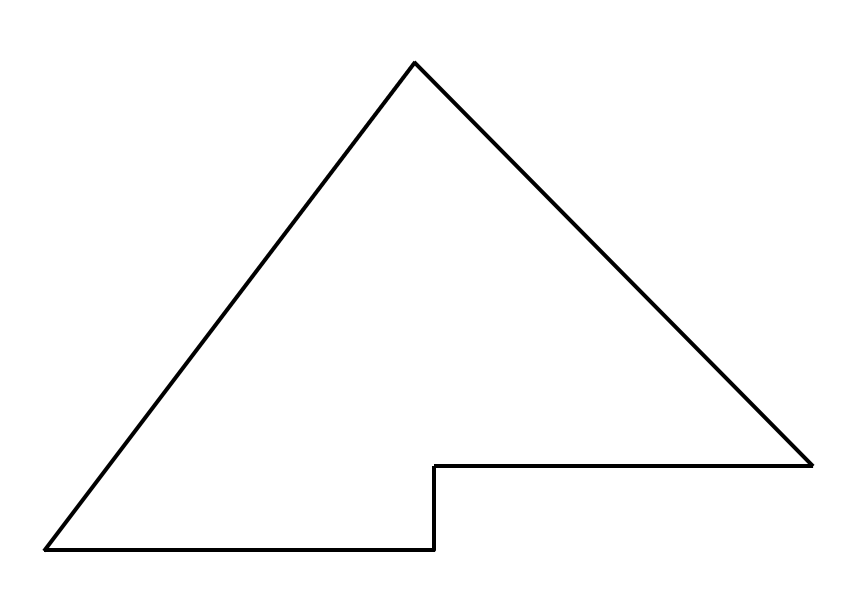
\includegraphics[height=1.3in]{heap}}
\caption{Heap}
\label{fig:heap}
\end{figure}
\section{Operations}
Assume the root \textbf{starts} at $a[1]$ rather than $a[0]$.
\\
Basic operations:
\begin{enumerate}
\item sink()/ sift\_down() - recursive
\item swim()/ sift\_up() - recursive
\item build()/ heapify() - bottom-up sink()
\end{enumerate}
\subsection{Sink (sift\_down)}
Core clue: compare parent to the \textit{larger} child. 
\begin{python}
def sink(self, idx):
    while 2*idx <= self.N:
        c = 2*idx
        if c+1 <= self.N and self.less(c, c+1):
            c += 1
        if not self.less(idx, c):
            return 

        self.swap(idx, c)
        idx = c
\end{python}

\subsection{Swim (sift\_up)}
Core clue: compare child to its parent. 
\begin{python}
def swim(self, idx):
    while idx > 1 and self.less(idx/2, idx):
        pi = idx/2
        self.swap(pi, idx)
        idx = pi
\end{python}
\subsection{Heapify}
Core clue: bottom-up sink().
\begin{python}
def heapify(self):
    for i in xrange(self.N/2, 0, -1):
        self.sink(i);
\end{python}
\runinhead{Complexity.} Heapifying \textbf{a sorted array} is the worst case for heap construction, because the root of each subheap considered sinks all the way to the bottom. The worst case complexity $\sim 2N$. 

Building a heap is $O(N)$ rather than $O(N \lg N)$. Intuitively, the deeper the level, the more the nodes, but the less the level to sink down. 

At most $\big\lceil\frac{n}{2^{h+1}}\big\rceil$ nodes of any height $h$.

Proof:
\begin{align*}
\because \sum_{i=0}^{+\infty} {ix^i} =\frac{x}{(1-x)^2} \\
\therefore \sum_{h=0}^{\lfloor\lg n\rfloor}{\Big\lceil\frac{n}{2^{h+1}}\Big\rceil
O(h)} &= O\Bigg(n\sum_{h=0}^{\lfloor\lg n\rfloor}{\frac{h}{2^h}}\Bigg) \\
&= O(n)
\end{align*}

\section{Implementation}
\subsection{General}
The self-implemented binary heap's index usually starts at 1 rather than 0. 

The array representation of heap is in \textbf{level-order}.

The main reason that we can use an array to represent the heap-ordered tree in a binary heap is because the tree is \textbf{complete}.

Suppose that we represent a BST containing N keys using an array, with $a[0]$ empty, the root at $a[1]$. The two children of $a[k]$ will be at $a[2k]$ and $a[2k+1]$. Then, the length of the array might need to be as large as $2^N$.

It is possible to have 3-heap. A 3-heap is an array representation (using 1-based indexing) of a complete 3-way tree.
The children of $a[k]$ are $a[3k-1]$, $a[3k]$, and $a[3k+1]$.
\begin{figure}[hbtp]
\centering
\subfloat{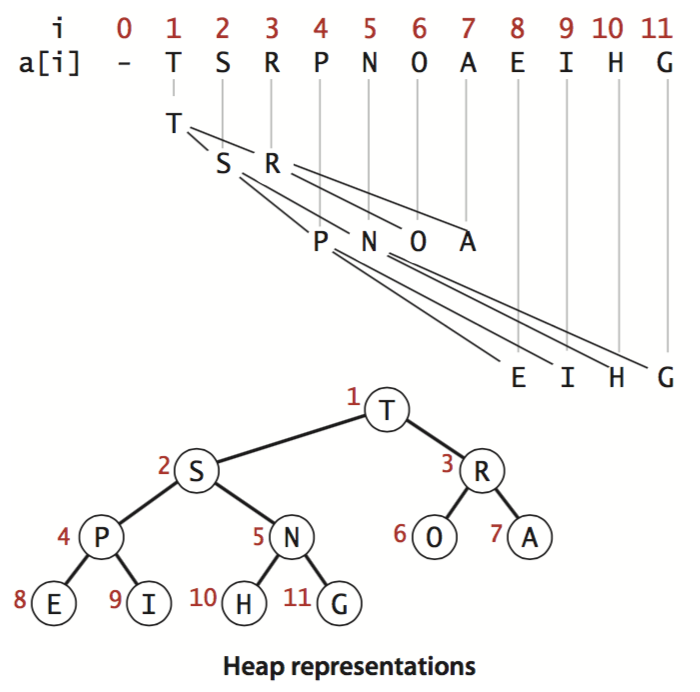
\includegraphics[scale=.90]{heapRepr}}
\caption{Heap representation}
\label{fig:heap} 
\end{figure}

\subsection{Python Heapq}
Python only has built in min-heap. To use max-heap, you can: 
\begin{enumerate}
\item Invert the number: 1 becomes -1.
(usually the best solution)\item Wrap the data into another class and override \textbf{comparators}: \_\_cmp\_\_ or \_\_lt\_\_
\end{enumerate}

The following code presents the wrapping method:
\begin{python}
class Value(object):
    def __init__(self, val):
        self.val = val
        self.deleted = False  # lazy delete 

    def __cmp__(self, other):
        # Reverse order by height to get max-heap
        assert isinstance(other, Value)
        return other.val - self.val
\end{python}

Normally the deletion by value in Python is $O(n)$, to achieve $O(\lg n)$ we can use \textbf{lazy deletion}. Before take the top of the heap, we do the following:
\begin{python}
while heap and heap[0].deleted:
    heapq.heappop(heap)
\end{python}
\subsection{Java Priority Queue}
\begin{java}
// min-heap
PriorityQueue<Integer> pq = new PriorityQueue<>(
    (o1, o2) -> o1-o2
);

// max-heap
PriorityQueue<Integer> pq = new PriorityQueue<>(
    (o1, o2) -> o2-o1
);
\end{java}

\chapter{Tree}

\section{Binary Tree}
\subsection{Introductions}
\runinhead{Get parent ref.} To get a parent reference (implicitly), \textit{return the Node} of the current recursion function to its parent to maintain the path. Sample code:
\begin{java}
Node deleteMin(Node x) {
    if (x.left == null) return x.right;
    x.left = deleteMin(x.left);
    // x.count = 1+size(x.left)+size(x.right);
    return x;
}
\end{java}
\runinhead{Construct path from root to target.} To search a node in binary tree (not necessarily BST), use dfs:
\begin{python}
def dfs(self, root, t, path, found):
    # post-call check
    if not root: return        
    if found[0]: return 

    path.append(root)
    if root == t:
        found[0] = True

    self.dfs(root.left, t, path, found)
    self.dfs(root.right, t, path, found)
    if not found[0]:
        path.pop()  # 1 pop() corresponds to 1 append()
\end{python}
The `found` is a wrapper for boolean to keep it referenced by all calling stack. 

\runinhead{Lowest common ancestor.} In BST, the searching is straightforward. In normal binary tree, construct the path from root to $node_1$ and $node_2$ respectively, and \textbf{diff} the two paths.

\runinhead{Find all paths.} Find all paths from root to leafs. For every currently visiting node, add itself to path; search left, search right and pop itself. Record current result when reaching the leaf.
\begin{python}
def dfs_path(self, cur, path, ret):
    if not cur: return

    path.append(cur)
    if not cur.left and not cur.right:
        ret.append("->".join(map(lambda x: str(x.val), path)))

    self.dfs_path(cur.left, path, ret)
    self.dfs_path(cur.right, path, ret)
    path.pop()
\end{python}
\subsection{Morris Traversal} 
Traversal with O(1) space. \footnote{\href{http://www.cnblogs.com/AnnieKim/archive/2013/06/15/MorrisTraversal.html}{ref}}

Time complexity $O(3n).$ - find \pyinline{pre} twice, \pyinline{cur} traverse once. \begin{figure}[hbtp]
\centering
\subfloat{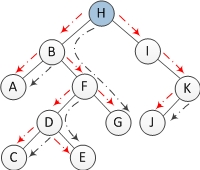
\includegraphics[height=0.9in]{morris_time}}
\caption{Morris traversal time complexity}
\label{fig:morrisTime}
\end{figure}

\subsubsection{Inoder}
Assign the current node's in-order predecessor's right child to itself (threading). Two ptr \pyinline{cur}, \pyinline{pre}. 

Process:
\begin{enumerate}
\item If no left, \textit{consume} \pyinline{cur}, go right 
\item If left, find in-order predecessor \pyinline{pre}
\begin{enumerate}
\item If no thread (i.e. no \pyinline{pre} right child), assign it to \pyinline{cur}; go left
\item If thread, \textit{consume} \pyinline{cur}, go right. ($\equiv$ no left). 
\end{enumerate}
\end{enumerate}

\begin{figure}[hbtp]
\centering
\subfloat{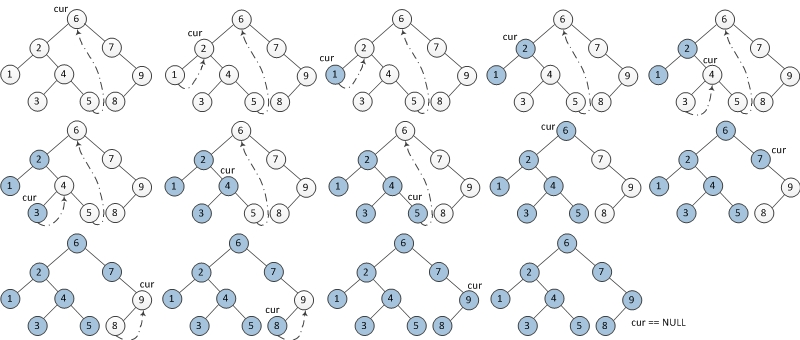
\includegraphics[height=1.6in]{morris_inorder}}
\caption{Morris inorder traversal}
\label{fig:morrisInorder}
\end{figure}
\newpage
Code:
\begin{python}
def morris_inorder(self, root):
    cur = root
    while cur:
        if not cur.left:
            self.consume(cur)
            cur = cur.right
        else:
            pre = cur.left
            while pre.right and pre.right != cur:
                pre = pre.right

            if not pre.right:
                pre.right = cur
                cur = cur.left
            else:
                pre.right = None
                self.consume(cur)
                cur = cur.right
\end{python}
\subsubsection{Preoder}
Similar to inorder. 

Process:
\begin{enumerate}
\item If no left, \textit{consume} \pyinline{cur}, go right 
\item If left, find in-order predecessor \pyinline{pre}
\begin{enumerate}
\item If no thread (i.e. no \pyinline{pre} right child), assign it to \pyinline{cur}; \textit{consume} \pyinline{cur}, go left
\item If thread, go right. ($\equiv$ no left, but no \textit{consume}, since consume before). 
\end{enumerate}
\end{enumerate}

\subsubsection{Postorder}
More tedious.
\begin{figure}[hbtp]
\centering
\subfloat{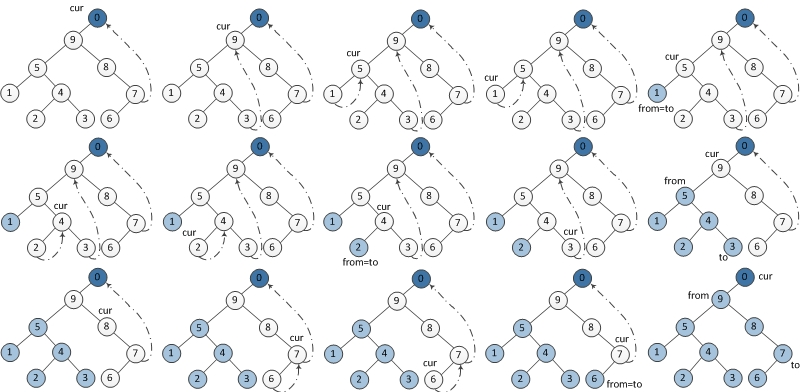
\includegraphics[height=1.6in]{morris_postorder}}
\caption{Morris inorder traversal}
\label{fig:morrisInorder}
\end{figure}

TODO

\section{Binary Search Tree (BST)}
\runinhead{Array and BST.}Given either the \textbf{preorder} or \textbf{postorder} (but not inorder) traversal of a BST containing N distinct keys, it is possible to reconstruct the shape of the BST. 
\subsection{Rank}
\runinhead{Calculates rank.}
\begin{enumerate}
\item When inserting: 
  \begin{enumerate}
  \item insert to an existing node: \pyinline{node.cnt_this += 1}
  \item insert to left subtree: \pyinline{node.cnt_left += 1}
  \item insert to right subtree: do nothing. 
\end{enumerate}
\item When querying rank:
  \begin{enumerate}
  \item query equals current node: \pyinline{return node.cnt_left}
  \item query goes to \textbf{left} node: \pyinline{return rank(node.left, val)};
  \item query goes to \textbf{right} node: \pyinline{return node.cnt_left} \pyinline{+ node.cnt_this + rank(node.right, val)}
  \end{enumerate}
Notice that the \pyinline{rank} calculates a val's rank in a subtree.
\end{enumerate}

\runinhead{Count of smaller number before itself.} Given an array $A$. For each element $A_i$ in the array, count the number of element before this element $A_i$ is smaller than it and return count number array. Average $O(n \log n)$
\\
Clues:
\begin{enumerate}
\item Put $A[:i+1]$ into a BST; so as to count the rank of $A[i]$ in the BST
\end{enumerate}
Codes:
\begin{python}
class Node(object):
  def __init__(self, val):
    """Records the left subtree size"""
    self.val = val
    self.cnt_left = 0
    self.cnt_this = 0
    self.left, self.right = None, None


class BST(object):
  def __init__(self):
    self.root = None

  def insert(self, root, val):
    """
    :return: subtree's root after insertion
    """
    if not root:
      root = Node(val)

    if root.val == val:
      root.cnt_this += 1
    elif val < root.val:
      root.cnt_left += 1
      root.left = self.insert(root.left, val)
    else:
      root.right = self.insert(root.right, val)

    return root

  def rank(self, root, val):
    """
    Rank in the root's subtree
    :return: number of items smaller than val
    """
    if not root:
      return 0
    if root.val < val:
      return (root.cnt_this+root.cnt_left+
              self.rank(root.right, val))
    elif root.val == val:
      return root.cnt_left
    else:
      return self.rank(root.left, val)


class Solution(object):
  def countOfSmallerNumberII(self, A):
    tree = BST()
    ret = []
    for a in A:
      tree.root = tree.insert(tree.root, a)
      ret.append(tree.rank(tree.root, a))

    return ret
\end{python}
Notice: if worst case $O(n \log n)$ is required, need to use Red-Back Tree - Section \ref{rbtree}. However, there is a more elegant way using Segment Tree - Section \ref{segmentTreeInversionCount}.


\subsection{Range search}
\runinhead{1-d range count}
\begin{java}
int size(Key lo, Key hi) {
    if (contains(hi)) return rank(hi)-rank(lo)+1;
    else              return rank(hi)-rank(lo);
}
\end{java}

\runinhead{Closest value} Find the value in BST that is closet to the \pyinline{target}.
\\
Clues:
\begin{enumerate}
\item Find the value just $\leq$ the target.
\item Find the value just $\geq$ the target.
\end{enumerate}
\
\\
Code for finding either the lower value or higher value:
\begin{python}
def find(self, root, target, ret, lower=True):
  """ret: result container"""
  if not root: return

  if root.val == target:
    ret[0] = root.val
    return

  if root.val < target:
    if lower:
      ret[0] = max(ret[0], root.val)

    self.find(root.right, target, ret, lower)
  else:
    if not lower:
      ret[0] = min(ret[0], root.val)

    self.find(root.left, target, ret, lower)
\end{python}

\runinhead{Closet values} Find $k$ values in BST that are closet to the \pyinline{target}.
\\\\
Clues:
\begin{enumerate}
\item Find the predecessors $\triangleq \{node | node.value \leq target\}$. Store in the stack. 
\item Find the successors $\triangleq \{node | node.value \geq target\}$. Store in the stack.
\item Merge the predecessors and successors as in merge in MergeSort to get he $k$ values. 
\end{enumerate}
\
\\
Code for finding the predecessors:
\begin{python}
def predecessors(self, root, target, stk):
  if not root: return

  self.predecessors(root.left, target, stk)
  if root.val <= target:
    stk.append(root.val)
    self.predecessors(root.right, target, stk)
\end{python}


\section{Binary Index Tree (BIT)}\label{BIT}
\subsection{Introduction}
Compared to Segment Tree \ref{section:segmentTree}, BIT is shorter and more elegant. BIT can do most of things that Segment Tree can do and it is easier to code. BIT updates and queries $$i\rightarrow prefixSum$$ in $O(\log n)$ time; however, BIT CANNOT query $$prefixSum \rightarrow i$$
\subsection{Implementation}
Given an array $A$ of length $n $ starting from $1$. prefix sum $s[i]\triangleq A_1+...+A_i$. BIT uses binary to maintain the array of prefix sum for querying and updating. For $i$-th node in the BIT, 
$$
N[i]=A_{j+1}+...+A_i
$$
, where $j=i-lowbit(i)$, i.e. set $i$'s lowest bit 1 to 0. $lowbit(i)$ can be defined as \pyinline{return i & -i}, using 2's complement. Notice that the summation ends with $A_i$ since easier to \pyinline{set}.

For the range, we use $(j, i]$ here instead of $[j, i)$ since more elegant for \pyinline{get(i)} and \pyinline{set(i)}
\\\\
Clues:
\begin{enumerate}
\item Binary 
\item Low bit
\item BIT uses array index starting from \textbf{1}, because 0 doesn't have $lowbit$.
\end{enumerate}
\begin{figure}[hbtp]
\centering
\subfloat{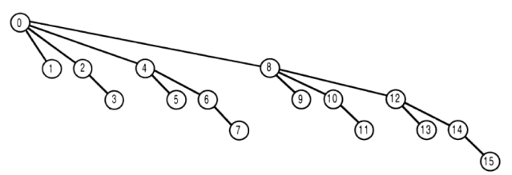
\includegraphics[height=1.1in]{BITget}}
\caption{Binary Indexed Tree \textit{get} Operation}
\label{fig:LABEL}
\end{figure}

\begin{figure}[hbtp]
\centering
\subfloat{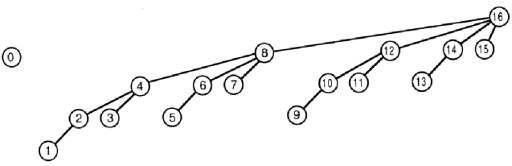
\includegraphics[height=1.05in]{BIT}}
\caption{Binary Indexed Tree \textit{set} Operation}
\label{fig:LABEL}
\end{figure}

Time complexity, longest update is along the leftmost branch, which takes $O(\log_2 n)$ (e.g. 1, 10, 100, 1000, 10000); longest query is along a branch starting with node with all 1's (e.g. 1111, 1110, 1100, 1000), which also takes $O(\log_2 n)$.
\newpage
Code:
\begin{python}
class BIT(object):
    def __init__(self, n):
        """BIT uses index starting from 1"""
        self.N = [0 for _ in xrange(n+1)]

    def lowbit(self, i):
        return i & -i

    def get(self, i):
        ret = 0
        while i > 0:
            ret += self.N[i]
            i -= self.lowbit(i)

        return ret
        
    def set(self, i, val):
        while i < len(self.N):
            self.N[i] += val
            i += self.lowbit(i)
\end{python}


\section{Segment Tree}\label{section:segmentTree}
\subsection{Introduction}
Segment Tree is specially built for \textit{range queries}. 

The structure of Segment Tree is a binary tree which each node has two attributes start and end denote an segment/interval. 

Notice that by practice, the interval is normally $[start, end)$ but sometimes it can be $[start, end]$, which depends on the question definition. 

Structure:  
\begin{lstlisting}[columns=flexible]
# a Count Segment Tree
                     [0, 4, count=3]
                     /             \
          [0,2,count=1]             [2,4,count=2]
          /         \               /            \
   [0,1,count=1] [1,2,count=0] [2,3,count=1], [3,4,count=1]
\end{lstlisting}
Variants:
\begin{enumerate}
\item Sum Segment Tree.
\item Min/Max Segment Tree.
\item Count Segment Tree. 
\end{enumerate}

For a Maximum Segment Tree, which each node has an extra value max to store the maximum value in this node's interval.

\subsection{Operations}
Segment Tree does a decent job for range queries.
\\
Components in Segment Tree operations:
\begin{enumerate}
\item Build
\item Query 
\item Modify
\item Search 
\end{enumerate}
Notice:
\begin{enumerate}
\item Only build need to change the start and end recursively.
\item Pre-check is preferred in recursive calls.
\end{enumerate}
Code: Notice the code has abstracted out segment tree functions of sum, min/max or count, by abstracting the subtree combine function to \pyinline{lambda}.
\begin{python}
DEFAULT = 0
f = lambda x, y: x+y


class Node(object):
    def __init__(self, start, end, m):
        self.start, self.end, self.m = start, end, m
        self.left, self.right = None, None


class SegmentTree(object):
    def __init__(self, A):
        self.A = A
        self.root = self.build_tree(0, len(self.A))

    def build_tree(self, s, e):
        """
        segment: [s, e)
        Either check s+1==e or have root.right 
        only if have root.left
        """
        if s >= e: return None
        if s+1 == e: return Node(s, e, self.A[s])

        left = self.build_tree(s, (s+e)/2)
        right = self.build_tree((s+e)/2, e)

        val = DEFAULT
        if left: val = f(val, left.m)
        if right: val = f(val, right.m)
        root = Node(s, e, val)
        root.left = left
        root.right = right

        return root

    def query(self, root, s, e):
        """
        :type root: Node
        """
        if not root:
            return DEFAULT

        if s <= root.start and e >= root.end:
            return root.m

        if s >= root.end or e <= root.start:
            return DEFAULT

        l = self.query(root.left, s, e)
        r = self.query(root.right, s, e)
        return f(l, r)

    def modify(self, root, idx, val):
        """
        :type root: Node
        """
        if not root or idx >= root.end or idx < root.start:
            return

        if idx == root.start and idx == root.end-1:
            root.m = val
            self.A[idx] = val
            return

        self.modify(root.left, idx, val)
        self.modify(root.right, idx, val)

        val = DEFAULT
        if root.left:  val = f(val, root.left.m)
        if root.right: val = f(val, root.right.m)
        
        root.m = val
\end{python}
Concrete example - Count Segment Tree \ref{inversionReconstruct}. 

\newpage
\section{Trie}
\subsection{Basic}
Trie is aka radix tree, prefix tree. 
\begin{figure}[hbtp]
\centering
\subfloat{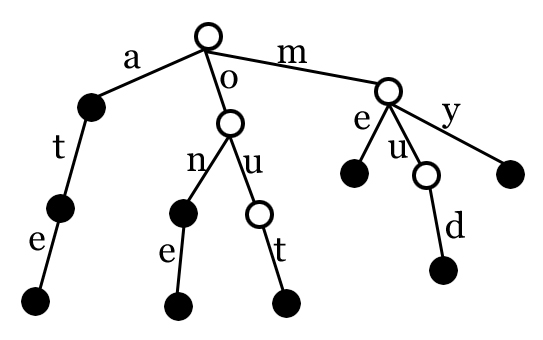
\includegraphics[scale=.30]{trie.jpg}}
\caption{Trie}
\label{fig:trie} 
\end{figure}
\runinhead{Notice:}
\begin{enumerate}
\item Children are stored in HashMap rather than ArrayList. 
\item self.word to stores the word and indicates whether a word ends at the current
node. 
\end{enumerate}
Codes:
\begin{python}
class TrieNode(object):
    def __init__(self, char):
        self.char = char
        self.word = None
        self.children = {}  # map from char to TrieNode


class Trie(object):
    def __init__(self):
        self.root = TrieNode(None)

    def add(self, word):
        word = word.lower()
        cur = self.root
        for c in word:
            if c not in cur.children:
                cur.children[c] = TrieNode(c)
            cur = cur.children[c]
        cur.word = word
\end{python}

\subsection{Advanced}
Implicit storage of word in TrieNode: 
\begin{enumerate}
\item Implicitly stores the current word. 
\item Implicitly stores the current char. 
\item When insert new word, do not override the existing TrieNode. A flag to indicate
whether there is a word ending here.
\end{enumerate}
\newpage
Code:
\begin{python}
class TrieNode:
    def __init__(self):
        """Implicit storage"""
        self.ended = False
        self.children = {}


class Trie:
    def __init__(self):
        self.root = TrieNode()

    def insert(self, word):
        cur = self.root
        for w in word:
            if w not in cur.children:   # not override
                cur.children[w] = TrieNode()
            cur = cur.children[w]

        cur.ended = True

    def search(self, word):
        cur = self.root
        for w in word:
            if w in cur.children:
                cur = cur.children[w]
            else:
                return False

        if not cur.ended:  # not ended here
            return False

        return True

    def startsWith(self, prefix):
        cur = self.root
        for w in prefix:
            if w in cur.children:
                cur = cur.children[w]
            else:
                return False

        return True
\end{python}
\subsection{Applications}
\begin{enumerate}
\item Word search in matrix.
\item Word look up in dictionary.
\end{enumerate}
        
     

\chapter{Balanced Search Tree}
\section{2-3 Search Tree}
\subsection{Insertion}
Insertion into a 3-node at bottom:
\begin{enumerate}
\item Add new key to the 3-node to create a temporary 4-node.
\item Move middle key of the 4-node into the parent (including root's parent).
\item Split the modified 4-node.
\item Repeat recursively up the trees as necessary.
\end{enumerate}
\begin{figure}[hbtp]
\centering
\subfloat{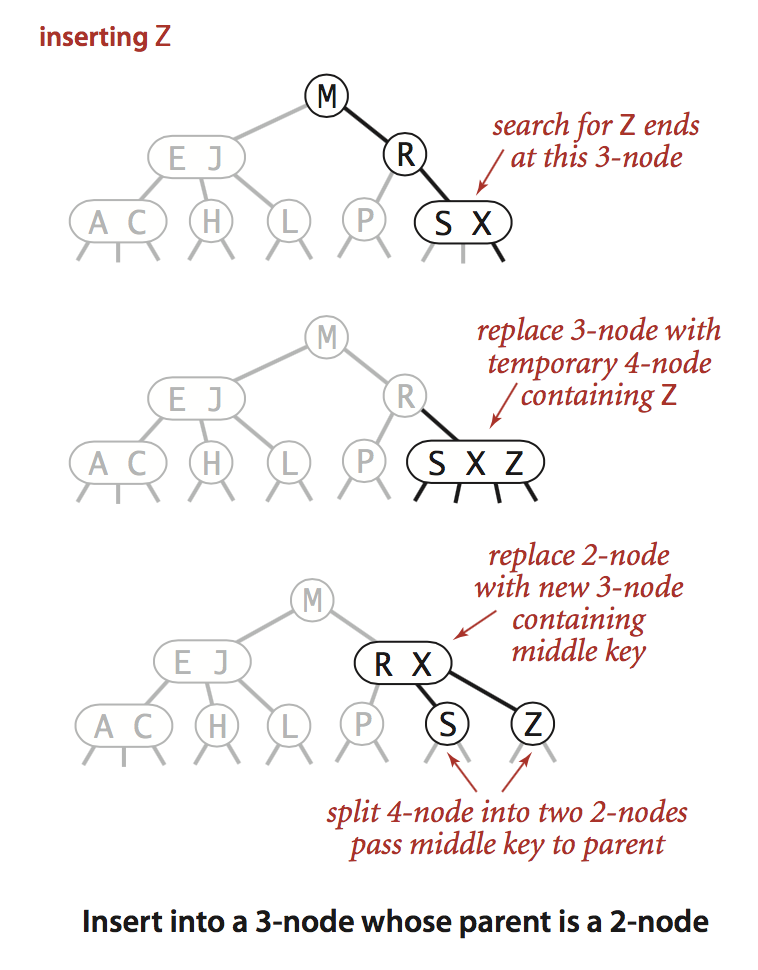
\includegraphics[scale=.8]{23insert1}}
\caption{Insertion 1}
\label{fig:LABEL}
\end{figure}

\begin{figure}[hbtp]
\centering
\subfloat{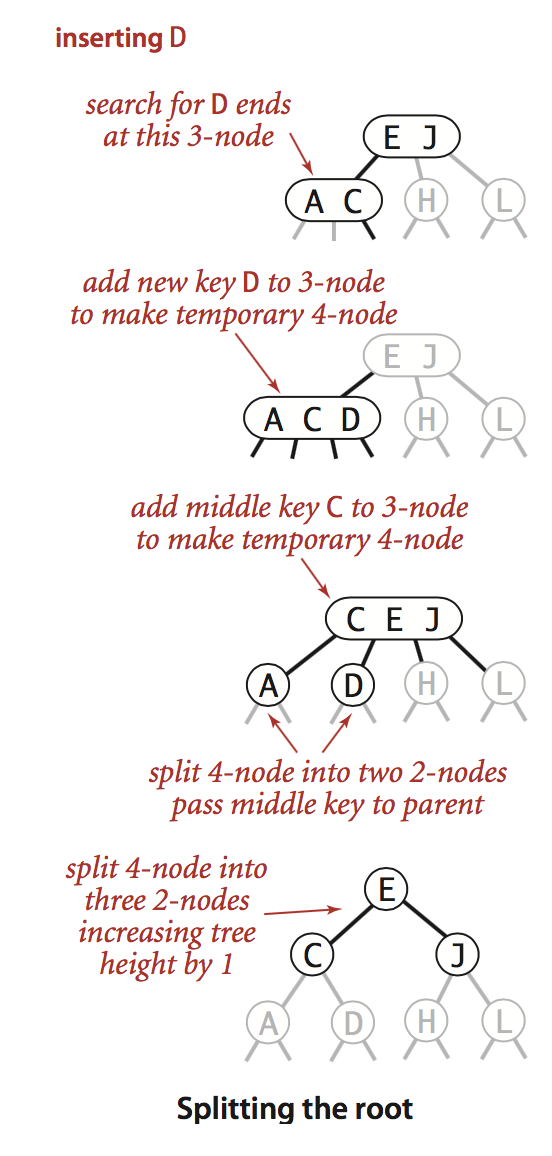
\includegraphics[scale=.8]{23insert2}}
\caption{insert 2}
\label{fig:LABEL}
\end{figure}

\subsection{Splitting}
Summary of splitting the tree. 
\begin{figure}[hbtp]
\centering
\subfloat{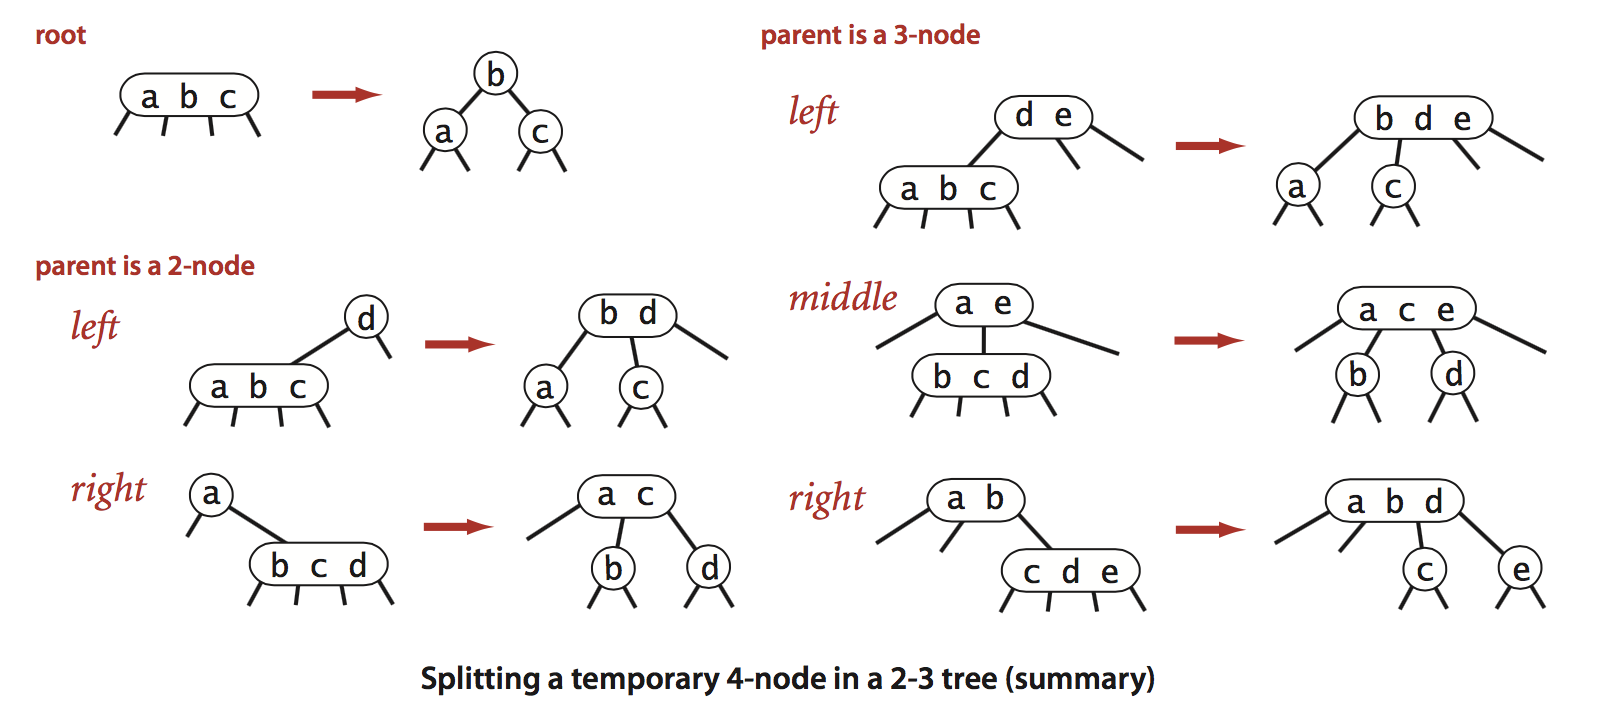
\includegraphics[scale=.65]{23splitting}}
\caption{Splitting temporary 4-ndoe summary}
\label{fig:splitting}
\end{figure}

\subsection{Properties}
When inserting a new key into a 2-3 tree, under which one of the following scenarios must the height of the 2-3 tree increase by one? When every node on the search path from the root is a 3-node

\section{Red-Black Tree}\label{rbtree}
\subsection{Properties}
Red-black tree is an implementation of 2-3 tree using \textbf{leaning-left red link}. \begin{figure}[hbtp]
\centering
\subfloat{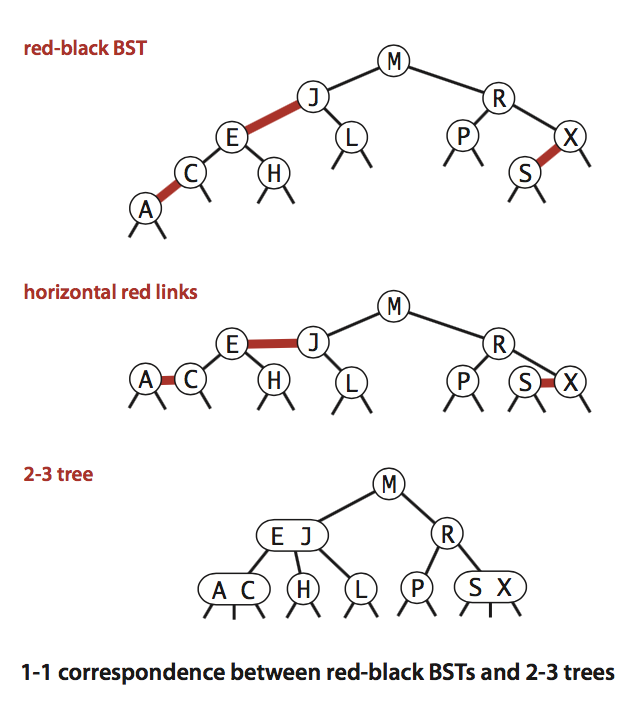
\includegraphics[scale=1.1]{rbtree11}}
\caption{RB-tree and 2-3 tree}
\label{fig:LABEL}
\end{figure}
The height of the RB-tree is at most $2\lg N$ where alternating red and black links. Red is the special link while black is the default link. 

\runinhead{Perfect black balance.}Every path from root to null link has the same number of black links.
\subsection{Operations}
\runinhead{Elementary operations:}
\begin{enumerate}
\item Left rotation: orient a (temporarily) right-leaning red link to lean left. Rotate leftward. 
\item Right rotation: orient a (temporarily) left-leaning red link to lean right. 
\item Color flip: Recolor to split a (temporary) 4-node. Rotate rightward. 
\end{enumerate}
\begin{figure}[hbtp]
\centering
\subfloat{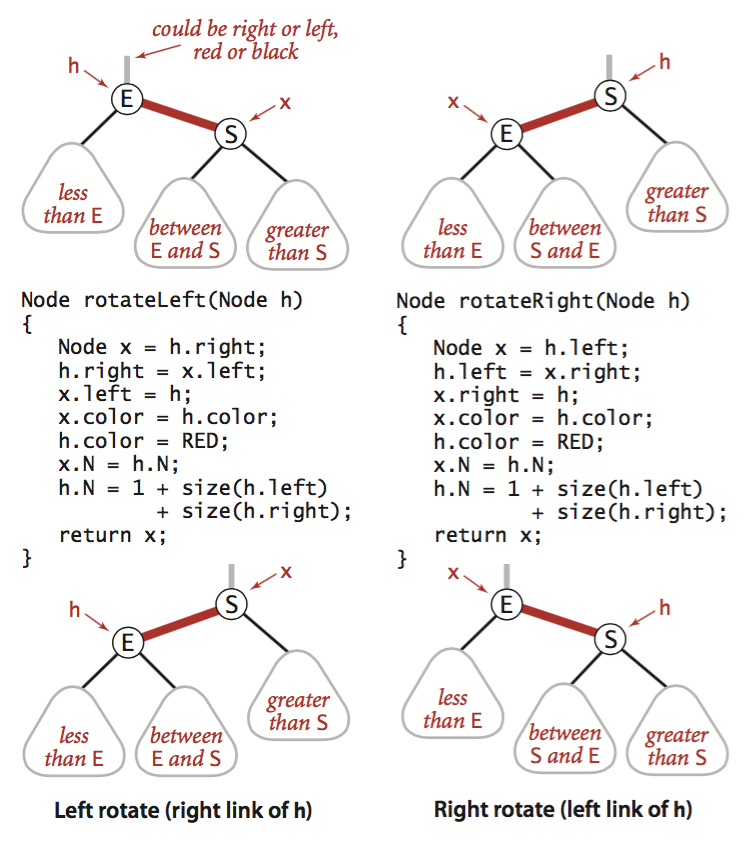
\includegraphics[scale=1.20]{rbrotate}}
\caption{Rotate left/right}
\label{fig:LABEL}
\end{figure}

\begin{figure}[hbtp]
\centering
\subfloat{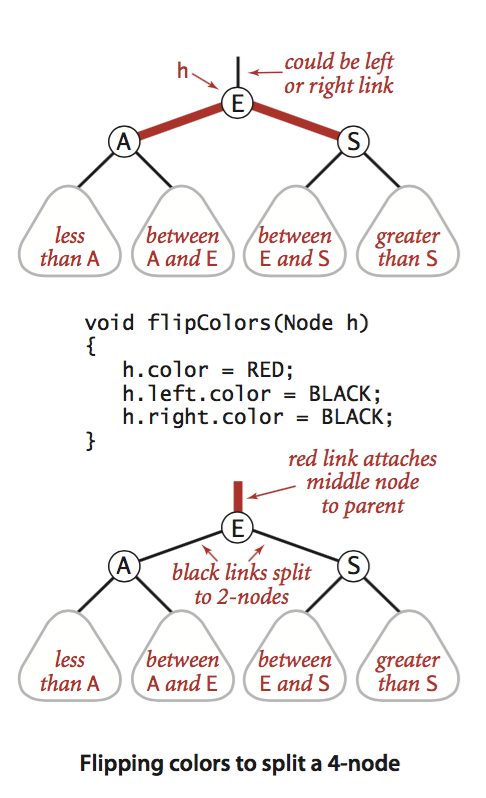
\includegraphics[scale=1.20]{rbflip}}
\caption{Flip colors}
\label{fig:LABEL}
\end{figure}

\runinhead{Insertion.} When doing insertion, from the child's perspective, need to have the information of current leaning direction and parent's color. Or from the parent's perspective - need to have the information of children's and grandchildren's color and directions.

For every new insertion, the node is always attached with red links. 

The following code is the simplest version of RB-tree insertion: 
\newpage
\begin{java}
Node put(Node h, Key key, Value val) {
  if (h == null)  // std red insert (link to parent).
    return new Node(key, val, 1, RED);
  int cmp = key.compareTo(h.key);
  if      (cmp < 0) h.left  = put(h.left,  key, val);
  else if (cmp > 0) h.right = put(h.right, key, val);
  else h.val = val; // pass

  if (isRed(h.right) && !isRed(h.left))    
    h = rotateLeft(h);
  if (isRed(h.left) && isRed(h.left.left)) 
    h = rotateRight(h);
  if (isRed(h.left) && isRed(h.right))     
    flipColors(h);

  h.N = 1+size(h.left)+size(h.right);
  return h; 
}
\end{java}

Rotate left, rotate right, then flip colors.

\runinhead{Illustration of cases.} Insert into a single 2-node: Figure-\ref{fig:rb_2}. Insert into a single 3-node: Figure-\ref{fig:rb_3}
\begin{figure}[t]
\begin{tabular}{cc}
  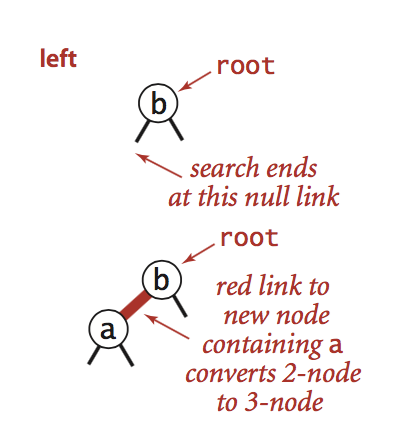
\includegraphics[height = 1.7in]{rb_left} &
  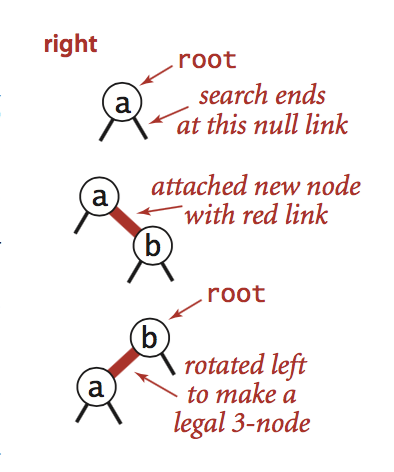
\includegraphics[height = 1.7in]{rb_right}\\
\end{tabular}
\caption{(a) smaller than 2-node (b) larger than 2-nod}
\label{fig:rb_2}
\end{figure}

\begin{figure}[t]
        \centerline{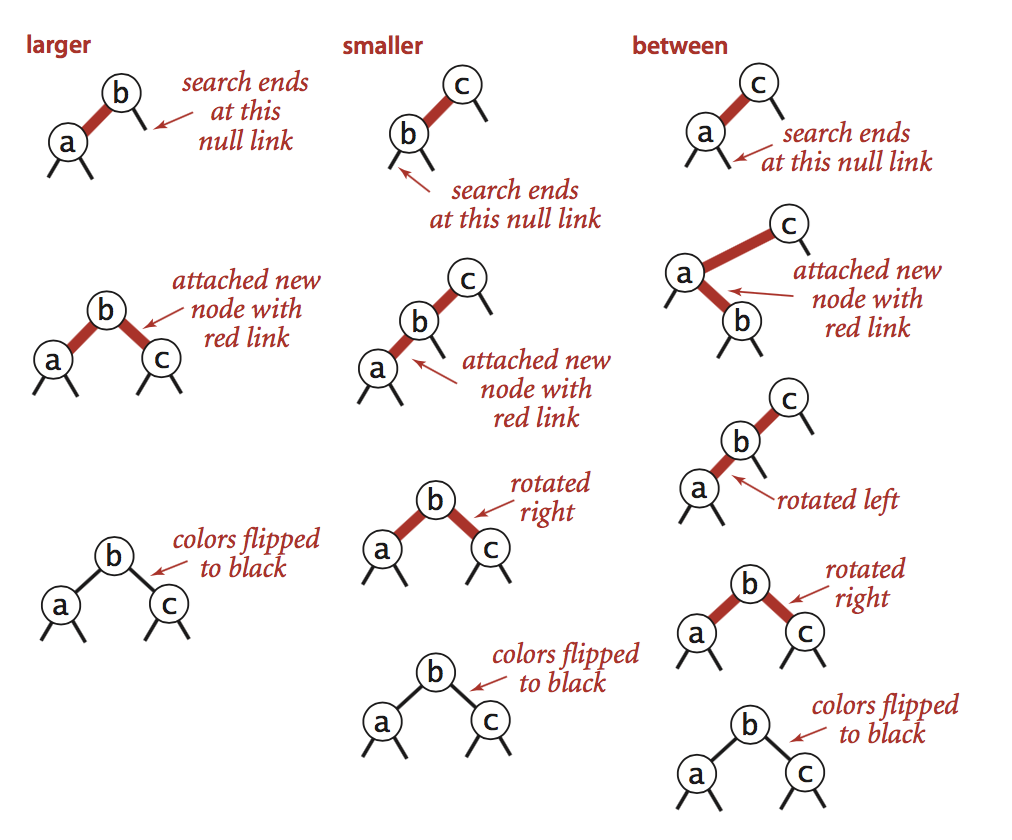
\includegraphics[height = 2.8in]{rb_3_left_right_btw}}
        \caption{(a) larger than 3-node (b) smaller than 3-node (c) between 3-node.}
    \label{fig:rb_3}
\end{figure}

\runinhead{Deletion.} Deletion is more complicated. 

\section{B-Tree}
B-tree is the generalization of 2-3 tree. 
\begin{figure}[hbtp]
\centering
\subfloat{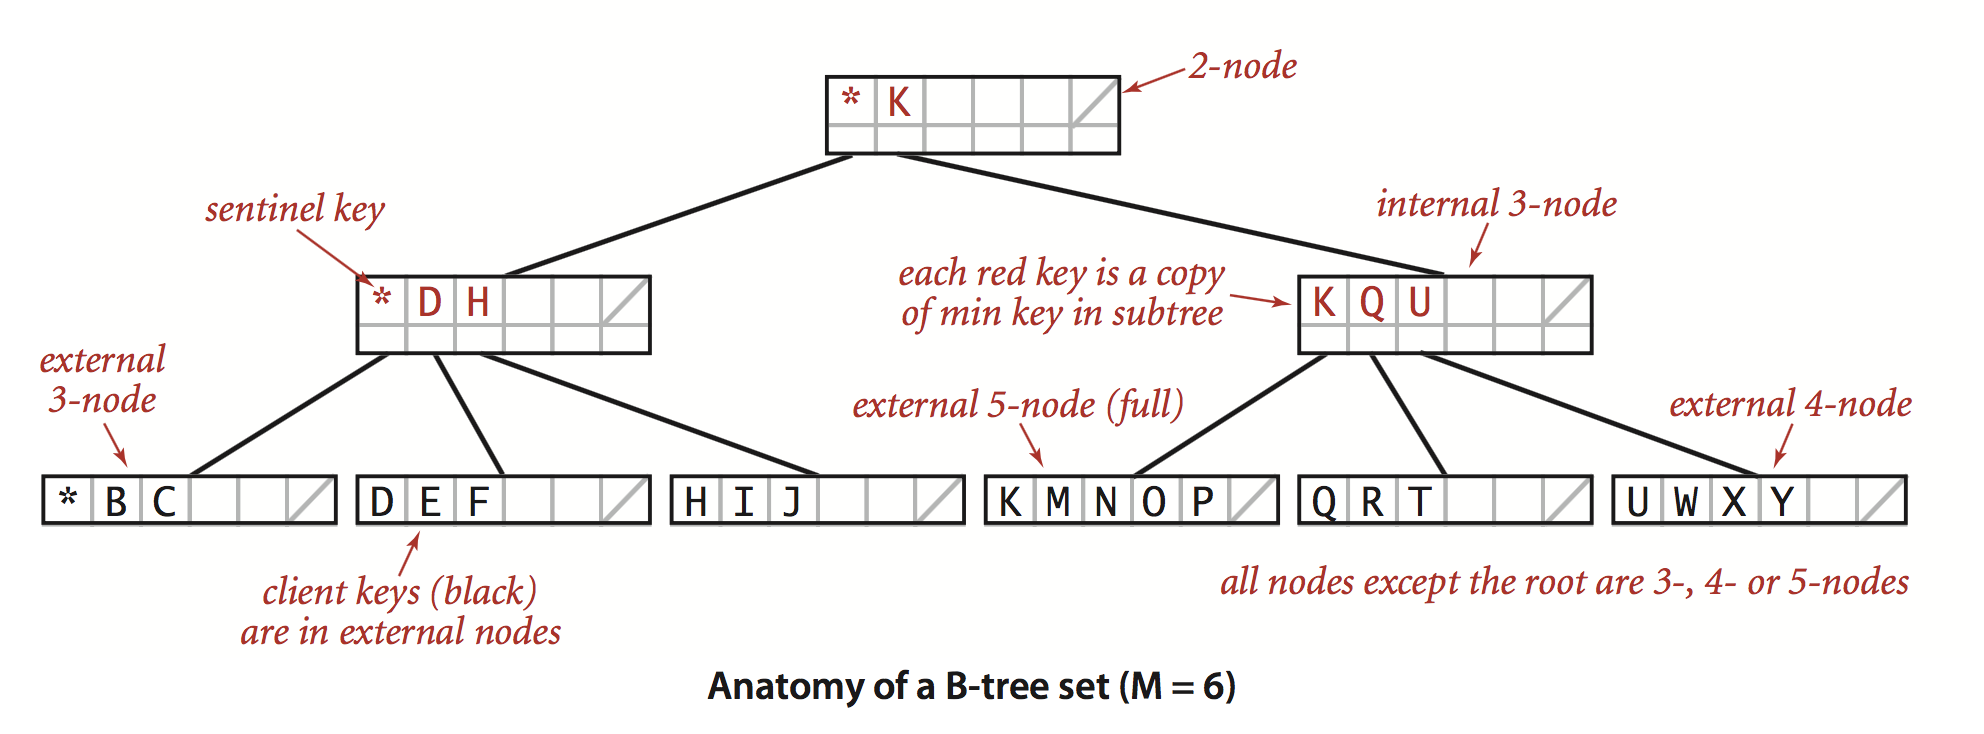
\includegraphics[scale=.50]{b-tree}}
\caption{B-Tree}
\label{fig:b-tree}
\end{figure}
\subsection{Basics}
Half-full principle: 

\begin{tabular}{lll}
\hline\noalign{\smallskip}
\textbf{Attrs} & \textbf{Non-leaf} & \textbf{Leaf} \\
\noalign{\smallskip}\hline\noalign{\smallskip}
Ptrs & \lceil\frac{n+1}{2}\rceil & \lfloor\frac{n+1}{2}\rfloor \\
\noalign{\smallskip}\hline\noalign{
\caption{Nodes at least half-full}
\end{tabular}

\subsection{Operations}
Core clues
\begin{enumerate}
\item \textbf{Invariant}: children balanced or left-leaning
\item \textbf{Split}: split half, thus invariant.
\item \textbf{Leaf-Up}: no delete, recursively move up the right node's first child;
thus invariant.
\item \textbf{Nonleaf-Up}: delete and recursively move up the left's last if left-leaning
or right's first if balanced; thus invariant. 
\end{enumerate}

\section{AVL Tree}
TODO

\section{Cartesian Tree}
\subsection{Basics}
Also known as max tree (or min tree). The root is the maximum number in the array. The left subtree and right subtree are the max trees of the subarray divided by the root number.
\begin{figure}[hbtp]
\centering
\subfloat{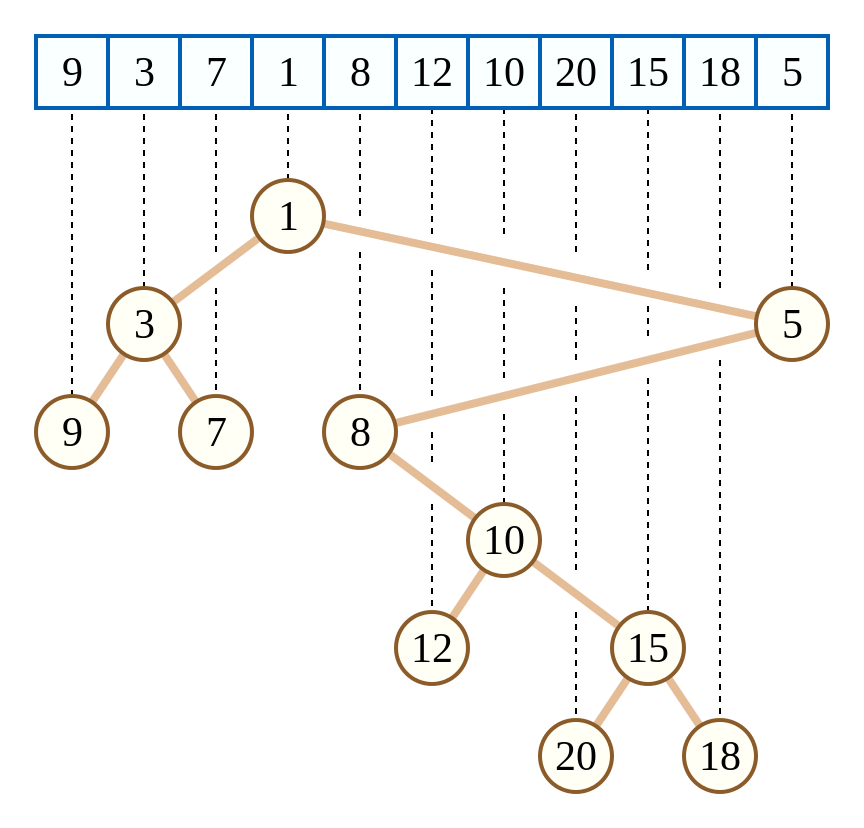
\includegraphics[scale=.60]{Cartesian_tree}}
\caption{Cartesian Tree}
\label{fig:cartesianTree}
\end{figure}
\begin{java}
Given [2, 5, 6, 0, 3, 1], the max tree is
     6
    / \
   5   3
  /   / \
 2   0   1
\end{java}
\runinhead{Construction algorithm.} Similar to all nearest smaller (or larger) values problem - Section \ref{allNearestSmaller}.

Core clues:
\begin{enumerate}
\item Use stack to maintain a \textit{strictly decreasing} stack, similar to find the all nearest large elements.
\itm Maintain the tree for currently scanning $A_i$ with the subarray $A[:i]$.
\begin{enumerate}
\item \rih{Left tree.} For each currently scanning node $A_i$, if ${stk}_{-1} \leq A_i$, then ${stk}_{-1}$ is the left subtree of $A_i$. Then pop the stack and iteratively look at ${stk}_{-1}$ again (previously ${stk}_{-2}$). Notice that the original left subtree of $A_i$ should become the right subtree of ${stk}_{-1} $, because the original left subtree appears later and satisfies the decreasing relationship.
\item \rih{Right tree.} In this stack, ${stk}_{-1} < {stk}_{-2}$ and ${stk}_{-1}$ appears later than ${stk}_{-2}$; thus ${stk}_{-1}$ is the right subtree of ${stk}_{-2}$. The strictly decreasing relationship of stack will be processed when popping the stack. 
\end{enumerate}
\end{enumerate}

$O(n)$ since each node on the tree is pushed and popped out from stack once.

\newpage
\begin{python}
def maxTree(self, A):
    stk = []
    for a in A:
        cur = TreeNode(a)
        while stk and stk[-1].val <= cur.val:
            pre = stk.pop()
            pre.right = cur.left
            cur.left = pre

        stk.append(cur)

    pre = None
    while stk:
        cur = stk.pop()
        cur.right = pre
        pre = cur

    return pre
\end{python}

Usually, min tree is more common. 
\subsection{Treap}
\rih{Randomized Cartesian tree}. Heap-like tree. It is a Cartesian tree in which each key is given a (randomly chosen) numeric priority. As with any binary search tree, the inorder traversal order of the nodes is the same as the sorted order of the keys.

\begin{figure}[hbtp]
\centering
\subfloat{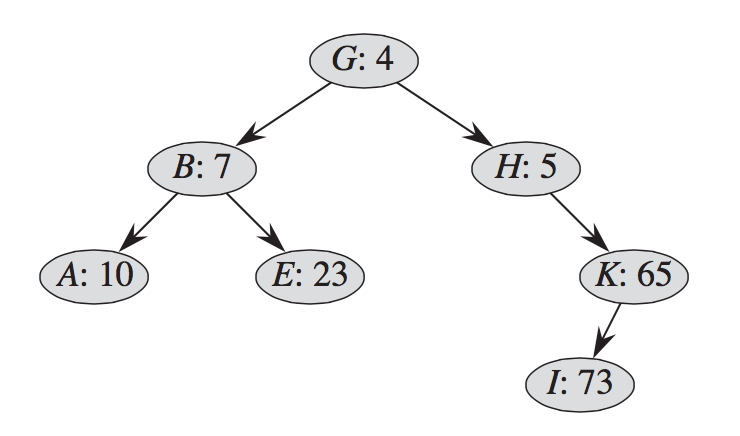
\includegraphics[scale=.80]{treap}}
\caption{Treap. Each node x is labeled with x.key: x.priority.}
\label{fig:treap}
\end{figure}

Construct a Treap for an array $A$ with index as the $x.key$ randomly chosen priority $x.priority$ $O(n)$. Thus support search, insert, delete into array (i.e. Treap) $O(\log n)$ on average. 

Insertion and deletion - need to perform \textit{rotations} to maintain the min-treap property. 


% algorithm
\chapter{Sort}


\section{Introduction}
List of general algorithms:
\begin{enumerate}
\item Selection sort: invariant
\begin{enumerate}
\item Elements to the left of $i$ (including $i$) are fixed and in ascending order (fixed and sorted).
\item No element to the right of $i$ is smaller than any entry to the left of $i$ ($A[i]  \leq\min(A[i+1:n])$.
\end{enumerate}
\item Insertion sort: invariant
\begin{enumerate}
\item Elements to the left of $i$ (including $i$) are in ascending order (sorted).
\item Elements to the right of $i$ have not yet been seen.
\end{enumerate}
\item Shell sort: h-sort using insertion sort.
\item Quick sort: invariant
\begin{enumerate}
\item $|A_p|..\leq..|..unseen..|..\geq..|$ maintain the 3 subarrays.
\end{enumerate}
\item Heap sort: compared to quick sort it is guaranteed $O(N \lg N)$, compared to merge sort it is $O(1)$ extra space. 
\end{enumerate}

\section{Algorithms}
\subsection{Quick Sort}
\subsubsection{Normal pivoting}\label{section:pivot}
The key part of quick sort is pivoting:
\begin{python}
def pivot(self, A, i, j):
    """
    pivoting algorithm:
    | p | closed set | open set |
    | closed set | p | open set |
    """
    p = i
    closed = p
    for ptr in xrange(i, j):
        if A[ptr] < A[p]:
            closed += 1
            A[ptr], A[closed] = A[closed], A[ptr]

    A[closed], A[p] = A[p], A[closed]
    return closed
\end{python}

Notice that this implementation goes $O(N^2)$ for arrays with all duplicates.

\textbf{Problem with duplicate keys}: it is important to stop scan at duplicate
keys (counter-intuitive); otherwise quick sort will goes $O(N^2)$ for the
array with all duplicate items, because the algorithm will put all items
equal to the $A[p]$ on \textbf{a single side}. 

Example: quadratic time to sort random arrays of 0s and 1s.

\subsubsection{Stop-at-equal pivoting}
Alternative pivoting implementation with optimization for duplicated keys:
\begin{python}
def pivot_optimized(self, A, lo, hi):
    """
    Fix the pivot as the 1st element
    Scan from left to right and right to left simultaneously
    Avoid the case that the algo goes O(N^2) with duplicated keys
    """
    p = lo
    i = lo
    j = hi
    while True:
        while True:
            i += 1
            if i >= hi or A[i] >= A[lo]:
                break
        while True:
            j -= 1
            if j < lo or A[j] <= A[lo]:
                break

        if i >= j:
            break

        A[i], A[j] = A[j], A[i]

    A[lo], A[j] = A[j], A[lo]
    return j

\end{python}
\subsubsection{3-way pivoting}
3-way pivoting: pivot the array into 3 subarrays: 

$|..\leq..|..=..|..unseen..|..\geq..|$ 
\begin{python}
def pivot_3way(self, A, lo, hi):
    lt = lo-1  # pointing to end of array LT
    gt = hi  # pointing to the end of array GT (reversed)

    v = A[lo]
    i = lo  # scanning pointer
    while i < gt:
        if A[i] < v:
            lt += 1
            A[lt], A[i] = A[i], A[lt]
            i += 1
        elif A[i] > v:
            gt -= 1
            A[gt], A[i] = A[i], A[gt]
        else:
            i += 1

    return lt+1, gt
\end{python}
\subsection{Merge Sort}
TODO
\section{Properties}
\subsection{Stability}
Definition: a stable sort preserves the \textbf{relative order of items with equal keys} (scenario: sorted by time then sorted by location). 

Algorithms:
\begin{enumerate}
\item Stable
\begin{enumerate}
\item Merge sort
\item Insertion sort
\end{enumerate} 
\item Unstable
\begin{enumerate}
\item Selection sort
\item Shell sort
\item Quick sort
\item Heap sort
\end{enumerate}
\end{enumerate}
\textbf{Long-distance swap} operation is the key to find the unstable case during sorting. 
\begin{figure}[hbtp]
\centering
\subfloat{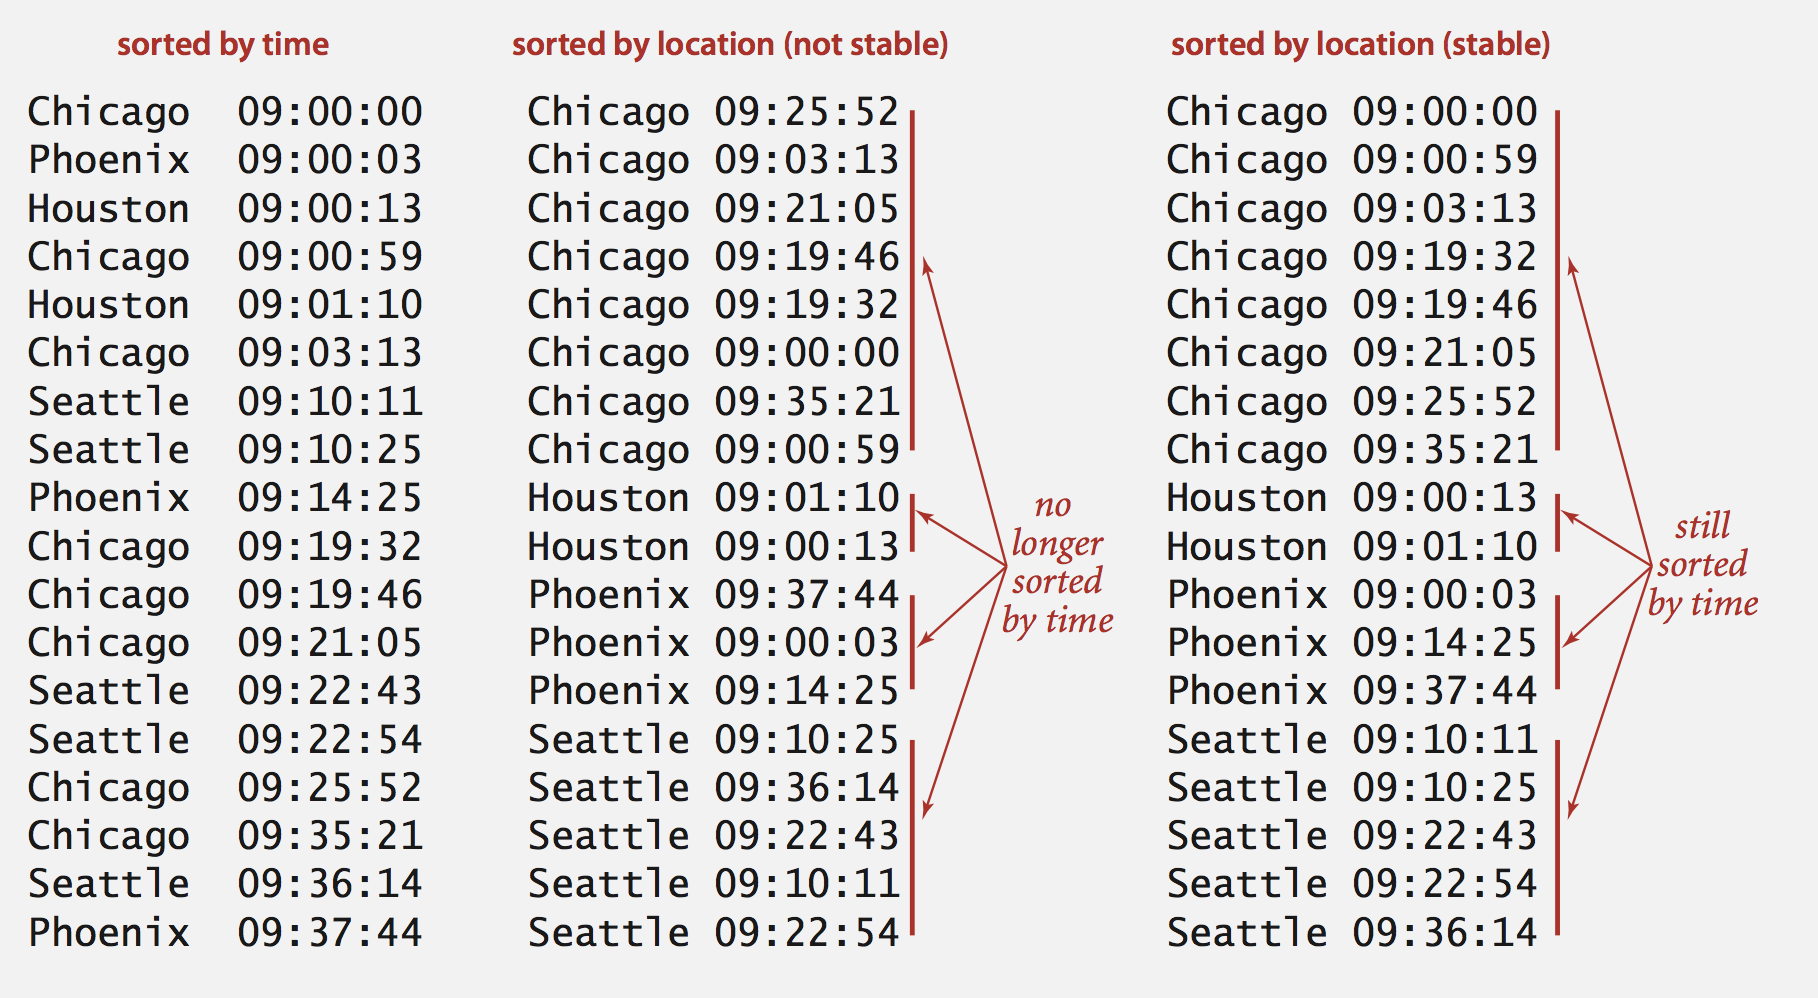
\includegraphics[scale=.50]{stable_sort}}
\caption{Stale sort vs. unstable sort}
\label{fig:trie} 
\end{figure}

\subsection{Sort Applications}
\begin{enumerate}
\item Sort
\item Partial quick sort (selection), k-th largest elements 
\item Binary search
\item Find duplicates 
\item Graham scan
\item Data compression
\end{enumerate}

\subsection{Considerations}
\begin{enumerate}
\item Stable?
\item Distinct keys?
\item Need guaranteed performance?
\item Linked list or arrays?
\item Caching system? (reference to neighboring cells in the array? 
\item Usually randomly ordered array?
(or partially sorted?)\item Parallel?
\item Deterministic?
\item Multiple key types?
\end{enumerate}

$O(N\lg N)$ is the lower bound of comparison-based sorting; but for other
contexts, we may not need $O(N \lg N)$:
\begin{enumerate}
\item Partially-ordered arrays: insertion sort to achieve $O(N)$. \textbf{Number of inversions}: 1 inversion $=$ 1 pair of keys that are out
of order.
\item Duplicate keys
\item Digital properties of keys: radix sort to achieve $O(N)$.
\end{enumerate}

\subsection{Summary}
\begin{figure}[hbtp]
\centering
\subfloat{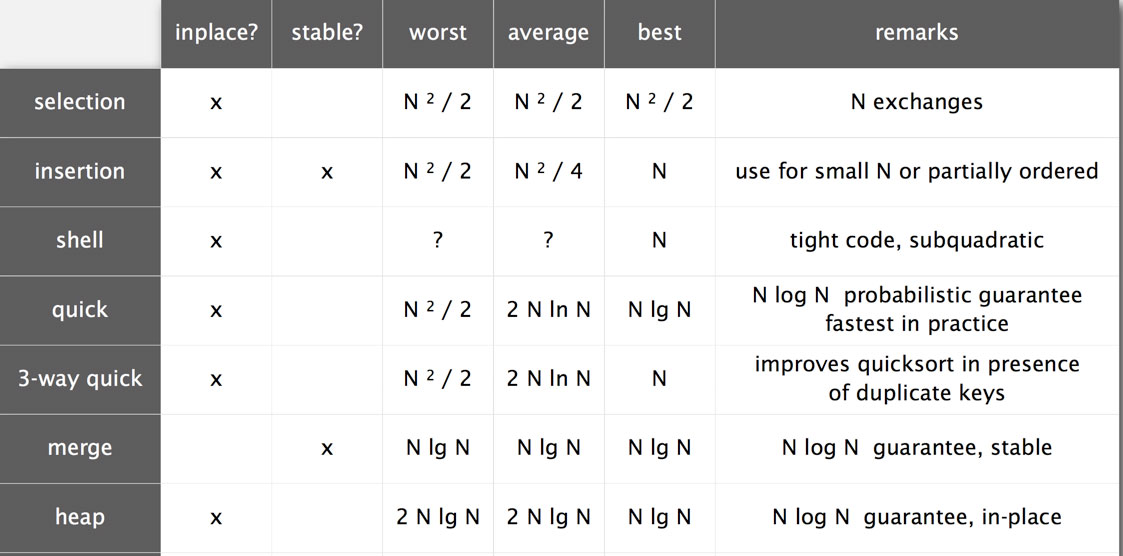
\includegraphics[scale=0.80]{sort_summary}}
\caption{Sort summary}
\label{fig:trie} 
\end{figure}
\section{Partial Quicksort}
\subsection{Find $m$ smallest}
\runinhead{Heap-based solution.} $O(n \log m)$
\runinhead{Partial Quicksort}  Then the $A[:m]$ is sorted $m$ smallest. The algorithm recursively sort the $A[i:j]$

The average time complexity is
\begin{eqnarray*}
F(n) = \left\{ \begin{array}{rl}
  F(\frac{n}{2})+O(n) &\mbox{// if $\frac{n}{2} \geq m$} \\
  2F(\frac{n}{2})+O(n) &\mbox{// otherwise}
       \end{array} \right.
\end{eqnarray*}
Therefore, the complexity is $O(n+m \log m)$.
\begin{python}
def partial_qsort(self, A, i, j, m):
    if i >= j: return

    p = self.pivot(A, i, j)
    self.partial_qsort(A, i, p, m)
    if p+1 >= m: return
    self.partial_qsort(A, p+1, j, m)
\end{python}

\subsection{Find $k$-th}
Use partial quick sort to find $k$-th smallest element in the unsorted array. The algorithm recursively sort the $A[i:j]$

The average time complexity is
\begin{align*}
F(n) &= F(n/2) + O(n) \\
&= O(n)
\end{align*}
\begin{python}
def find_kth(self, A, i, j, k):
    if i >= j: return
    
    p = self.pivot(A, i, j)
    if p == k: return A[p]
    if p > k:  return self.find_kth(A, i, p, k)
    else:      return self.find_kth(A, p+1, j, k)
\end{python}
Pivoting see section - \ref{section:pivot}.

\section{Inversion}
If $a_i > a_j$ but $i<j$, then this is considered as 1 Inversion. That is, for an element, the count of other elements that are \textit{larger} than the element but appear \textit{before} it. This is the default definition. 

There is also an alternative definition: for an element, the count of other elements that are \textit{samller} than the element but appear \textit{after} it. 

\subsection{MergeSort \& Inversion Pair}
MergeSort to calculate the reverse-ordered paris. The only difference from a normal
merge sort is that - when pushing the 2nd half of the array to the place, you calculate
the inversion generated by the element $A_2[i_2]$ compared to $A_1[i_1:]$.

\begin{python}
def merge(A1, A2, A):
  i1 = i2 =0
  ret = 0
  for i in xrange(len(A)):
    if i1 == len(A1):
      A[i] = A2[i2]
      i2 += 1
    elif i2 == len(A2):
      A[i] = A1[i1]
      i1 += 1
    else:
      # use array diagram to illustrate
      if A1[i1] > A2[i2]:  # push the A2 to A
        A[i] = A2[i2]
        i2 += 1
        # number of reverse-ordered pairs
        ret += len(A1) - i1
      else:
        A[i] = A1[i1]
        i1 += 1

  return ret

def merge_sort(a):
  n = len(a)
  if n == 1:
    return 0

  a1 = a[:n/2]
  a2 = a[n/2:]

  ret1 = merge_sort(a1)
  ret2 = merge_sort(a2)
  # merge not merge_sort
  ret = ret1+ret2+merge(a1, a2, a)  
  return ret
\end{python}

\subsection{Binary Index Tree \& Inversion Count}
Given $A$, calculate each element's inversion number. 

Construct a BIT (\ref{BIT}) with length $max(A)+1$. Let BIT maintains the index of values. Scan the element from left to right (or right to left depends on the definition of inversion number), and set the index equal val to 1. Use the prefix sum to get the inversion number.

\pyinline{get(end) - get(a)} get the count of number that appears \textit{before} $a$ (i.e. already in the BIT) and also \textit{larger} than $a$. 

Possible to extend to handle duplicate number. 
\\
Core clues:
\begin{enumerate}
\item BIT maintains \textbf{index of values} to count the number of at each value.
\item \pyinline{get(end) - get(a)} to get the inversion count of $a$.
\end{enumerate}
\begin{python}
def inversion(self, A):
    bit = BIT(max(A)+1)
    ret = []
    for a in A:
        bit.set(a, 1)  # += 1 if possible duplicate 
        inversion = bit.get(max(A)+1) - bit.get(a)
        ret.append(inversion)

    return ret
\end{python}

\subsection{Segment Tree \& Inversion Count}\label{segmentTreeInversionCount}
Compared to BIT, Segment Tree can process queries of both $idx \rightarrow sum$ and $sum \rightarrow idx$; while BIT can only process $idx \rightarrow sum$.

Core clues:
\begin{enumerate}
\item Segment Tree maintains \textbf{index of values} to count the number of at each value.
\item \pyinline{get(root, end) - get(root, a)} to get the inversion count of $a$.
\end{enumerate}
\begin{python}
class SegmentTree(object):
  def __init__(self):
    self.root = None

  def build(self, root, lo, hi):
    if lo >= hi: return
    if not root: root = Node(lo, hi)

    root.left = self.build(root.left, lo, (lo+hi)/2)
    if root.left: 
      root.right = self.build(root.right, (lo+hi)/2, hi)

    return root

  def set(self, root, i, val):
    if root.lo == i and root.hi-1 == root.lo:
      root.cnt_this += val
    elif i < (root.lo+root.hi)/2:
      root.cnt_left += val
      self.set(root.left, i, val)
    else:
      self.set(root.right, i, val)

  def get(self, root, i):
    if root.lo == i and root.hi-1 == root.lo:
      return root.cnt_left
    elif i < (root.lo+root.hi)/2:
      return self.get(root.left, i)
    else:
      return (
          root.cnt_left + root.cnt_this +
          self.get(root.right, i)
      )


class Solution(object):
  def _build_tree(self, A):
    st = SegmentTree()
    mini, maxa = min(A), max(A)
    st.root = st.build(st.root, mini, maxa+2)  
    # maxa+1 is the end dummy
    return st

  def countOfLargerElementsBeforeElement(self, A):
    st = self._build_tree(A)
    ret = []
    end = max(A)+1
    for a in A:
      ret.append(
          st.get(st.root, end) - st.get(st.root, a)
      )
      st.set(st.root, a, 1)

    return ret
\end{python}

\subsection{Reconstruct Array from Inversion Count}\label{inversionReconstruct}
Given a \textit{sorted} numbers with their associated inversion count (\# larger numbers before this element). $A[i].val$ is the value of the number, $A[i].inv$ is the inversion number. Reconstruct the original array $R$ that consists of each $A[i].val$.

Brute force can be done in $O(n^2)$. Put the $A[i].val$ into $R$ at an index/slot s.t. the \# \textit{empty} slots before it equals to $A[i].inv$.

\rih{BST}. Possible to use BST to maintain the empty slot indexes in the original array. Each node's rank indicates the count of empty indexes in its left subtree. But need to maintain the deletion.  

\rih{Segment Tree}. Use a segment tree to maintain the size of empty slots. Each node has a $start$ and a $end$ s.t slot indexes $\in [start, end)$. Go down to find the target slot, go up to decrement the size of empty slots. 

Reconstruction of array cannot use BIT since there is no map of $prefixSum \rightarrow i$.
\newpage
\begin{python}
class Node(object):
  def __init__(self, start, end, cnt):
    self.start = start
    self.end = end
    self.cnt = cnt

    self.left = None
    self.right = None

  def __repr__(self):
    return repr("[%d,%d)" % (self.start, self.end))


class SegmentTree(object):
  """empty space"""
  def __init__(self):
    self.root = None

  def build(self, start, end):
    """a node can have right ONLY IF has left"""
    if start >= end:
      return

    root = Node(start, end, end-start)
    root.left = self.build(start, (end+start)/2)
    if root.left: 
      root.right = self.build((start+end)/2, end)
    return root

  def find_delete(self, root, val):
    """
    :return: index
    """
    root.cnt -= 1
    if not root.left:
      return root.start
    elif root.left.cnt >= val:
      return self.find_delete(root.left, val)
    else:
      return self.find_delete(root.right, 
                              val - root.left.cnt)


class Solution(object):
  def reconstruct(self, A):
    st = SegmentTree()
    n = len(A)
    st.root = st.build(0, n)
    A = sorted(A, key=lambda x: x[0])
    ret = [0]*n
    for a in A:
      idx = st.find_delete(st.root, a[1]+1)
      ret[idx] = a[0]

    return ret

if __name__ == "__main__":
  A = [(5, 0), (2, 1), (3, 1), (4, 1,), (1, 4)]
  assert Solution().reconstruct(A) == [5, 2, 3, 4, 1]
\end{python}

\chapter{Search}

\section{Binary Search}
\runinhead{Variants:}
\begin{enumerate}
\item get the idx equal or just lower (floor)
\item get the idx equal or just higher (ceil)
\item \pyinline{bisect_left}
\item \pyinline{bisect_right} 
\end{enumerate}
\subsection{idx equal or just lower}
Binary search, get the idx of the element equal to or just lower than the target. The returned idx is the $A_{idx} \leq target$. It is possible to return $-1$. It is different from the \pyinline{bisect_lect}.

\runinhead{Core clues:}
\begin{enumerate}
\item To get ``equal'', \pyinline{return mid}.
\item To get ``just lower'', \pyinline{return lo-1}.
\end{enumerate}
$A_{idx} \leq target$.
\begin{python}
def bin_search(self, A, t, lo=0, hi=None):
    if hi is None: hi = len(A)
    
    while lo < hi:
        mid = (lo+hi)/2
        if A[mid] == t:  return mid
        elif A[mid] < t: lo = mid+1
        else:            hi = mid

    return lo-1
\end{python}
\subsection{idx equal or just higher}
$A_{idx} \geq target$.
\begin{python}
def bin_search(self, A, t, lo=0, hi=None):
    if hi is None: hi = len(A)
   
    while lo < hi:
        mid = (lo+hi)/2
        if A[mid] == t:  return mid
        elif A[mid] < t: lo = mid+1
        else:            hi = mid
        
    return lo
\end{python}
\subsection{bisect\_left}
Return the index where to insert item x in list A. So if t already appears in the list,
A.insert(t) will insert just before the \textit{leftmost} t already there.
\runinhead{Core clues:}
\begin{enumerate}
\item Move \pyinline{lo} if $A_{mid} < t$
\item Move \pyinline{hi} if $A_{mid} \geq t$
\end{enumerate}

\begin{python}
def bisect_left(A, t, lo=0, hi=None):
    if hi is None: hi = len(A)

    while lo < hi:
        mid = (lo+hi)/2
        if A[mid] < t: lo = mid+1   
        else:          hi = mid

    return lo
\end{python}

\subsection{bisect\_right}
Return the index where to insert item x in list A. So if t already appears in the list, A.insert(t) will insert just after the \textit{rightmost} x already there.
\runinhead{Core clues:}
\begin{enumerate}
\item Move \pyinline{lo} if $A_{mid} \leq t$
\item Move \pyinline{hi} if $A_{mid} > t$
\end{enumerate}
\begin{python}
def bisect_right(A, t, lo=0, hi=None):
    if hi is None: hi = len(A)

    while lo < hi:
        mid = (lo+hi)/2
        if A[mid] <= t: lo = mid+1
        else:           hi = mid 

    return lo
\end{python}
\section{Applications}
\subsection{Rotation}
\runinhead{Find Minimum in Rotated Sorted Array.} Three cases to consider:
\begin{enumerate}
\item Monotonous 
\item Trough 
\item Peak
\end{enumerate}

If the elements can be duplicated, need to detect and skip. 
\begin{python}
def findMin(self, A):
    lo = 0
    hi = len(A)
    mini = sys.maxint
    while lo < hi:
        mid = (lo+hi)/2
        mini = min(mini, A[mid])
        if A[lo] == A[mid]:  # JUMP
            lo += 1
        elif A[lo] < A[mid] <= A[hi-1]:
            return min(mini, A[lo])
        elif A[lo] > A[mid] <= A[hi-1]:  # trough
            hi = mid
        else:  # peak
            lo = mid+1

    return mini
\end{python}
\section{Combinations}
\subsection{Extreme-value problems}\label{extremeValueProblem}
\runinhead{Longest increasing subsequence.} Array $A$.

Clues:
\begin{enumerate}
\item \pyinline{MIN}: \textit{min} of index \textit{last} value of LIS of a particular \textit{len}.
\item \pyinline{RET}: result table, store the $\pi$'s idx (predecessor); (optional, to build the LIS, no need if only needs to return the length of LIS)
\item \pyinline{bin_search}: For each currently scanning index \pyinline{i}, if it smaller (i.e. $\neg$ increasing), to maintain the \pyinline{MIN}, binary search to find the position to update the min value. The \pyinline{bin_search} need to find the element $\geq$ to \pyinline{A[i]}.
\end{enumerate}
\newpage
\begin{python}
def LIS(self, A):
    n = len(A)
    MIN = [-1 for _ in xrange(n+1)]
    
    l = 1
    for i in xrange(1, n):
        if A[i] > A[MIN[l]]:
            l += 1
            MIN[l] = i
        else:
            j = self.bin_search(MIN, A, A[i], 1, l+1)
            MIN[j] = i

    return l
\end{python}
If need to return the LIS itself. 
\begin{python}
    for i in xrange(1, n):
        if A[i] > A[MIN[l]]:
            l += 1
            MIN[l] = i

            RET[i] = MIN[l-1]  # (RET)
        else:
            j = self.bin_search(MIN, A, A[i], 1, l+1)
            MIN[j] = i

            RET[i] = MIN[j-1] if j-1 >= 1 else -1  # (RET)

    # build the LIS (RET)
    cur = MIN[l]
    ret = []
    while True:
        ret.append(A[cur])
        if RET[cur] == -1: break
        cur = RET[cur]

    ret = ret[::-1]
    print ret
\end{python}

\section{High dimensional search}
\subsection{2D}
\runinhead{2D search matrix I.} $m\times n$ mat. Integers in each row are sorted from left to right. The first integer of each row is greater than the last integer of the previous row.
$$
\begin{bmatrix}
1 & 3 & 5 & 7 \\
10 & 11 & 16 & 20 \\
23 & 30 & 34 & 50 \\
\end{bmatrix}
$$

Row column search: starting at top right corner: $O(m+n)$.

Binary search: search rows and then search columns: $O(\log m + \log n)$.


\runinhead{2D search matrix II.} $m\times n$ mat. Integers in each row are sorted from
left to right. Integers in each column are sorted in ascending from top to bottom.
$$
\begin{bmatrix}
1&   4&  7& 11& 15 \\
2&   5&  8& 12& 19 \\
3&   6&  9& 16& 22 \\
10& 13& 14& 17& 24 \\
18& 21& 23& 26& 30 \\
\end{bmatrix}
$$ 

Row column search: starting at top right corner: $O(m+n)$.

Binary search: search rows and then search columns, but upper bound row and lower bound row: 

$$O\big(\min(n\log m, m\log n)\big)$$

\chapter{Array}
\section{Circular Array}
This section describes common patterns for solving problems with circular arrays.

Normally, we should solve the linear problem and circular problem differently.

\subsection{Circular max sum}
Linear problem can be solved linear with dp algorithm for maximum subarray sum - Section \ref{dpSequence}. 

The circular sum should use dp. 

Problem description: Given an integer array, find a continuous rotate subarray where the sum of numbers is the biggest. Return the index of the first number and the index of the last number. 
\runinhead{Core clues:}
\begin{enumerate}
\item \textbf{State definitions}: 

Construct left max sum $L_i$ for max sum over the $[0..i]$ with subarray starting at 0 (\textit{forward} starting from the left side). 

Construct right max sum $R_i$ for max sum over the indexes $[i+1..n -1]$, with subarray ending at -1 (\textit{backward} starting from the right side). 

Notice, for the two max sums, the index ends AT or BEFORE $i$.

\item \textbf{Transition functions:}
\begin{align*}
L_i = \max\Big(L_{i-1}, sum(A[:i])\Big) \\ 
R_i = \max\Big(R_{i+1}, sum(A[i:])\Big)
\end{align*}

\item \textbf{Global result}: 
$$maxa = \max(R_i+L_{i-1}, \forall i)$$
\end{enumerate}

\subsection{Non-adjacent cell}
Maximum sum of non-adjacent cells in an array $A$.

To solve circular non-adjacent array problem in linear way, we should consider 2 cases:
\begin{enumerate}
\item Not consider the $A[1]$
\item Not consider the $A[-1]$ 
\end{enumerate}
and solve them using linear maximum sum of non-adjacent cells separately  - Section \ref{dpSequence}. 
\subsection{Binary search}
Searching for an element in a circular sorted array. Half of the array is sorted while the other half is not.
\begin{enumerate}
\item If $A[0] < A[mid]$, then all values in the first half of the array are sorted.
\item If $A[mid] < A[-1]$, then all values in the second half of the array are sorted.
\item Then \textit{derive and decide} whether to got the \textbf{sorted half} or the \textbf{unsorted half}.
\end{enumerate}
\section{Voting Algorithm}
\subsection{Majority Number}
\subsubsection{$\frac{1}{2}$ of the Size}
Given an array of integers, the majority number is the number that occurs more than half of the size of the array. 

Algorithm: Majority Vote Algorithm. Maintain a counter to count how many times the majority number appear more than any other elements before index $i$ and after re-initialization. Re-initialization happens when the counter drops to 0. 

Proof: assuming there is a majority number $x$, if at the index $i$, the current count is $j$ and the current counter does not capture the majority number, there are less than $\frac{i-j}{2}$ $x$, thus there are more than $\frac{n-i+j}{2}$ $x$ after the index $i$. The $j$ $x$ beats against the counter and $\frac{n-i-j}{2}$ $x$ will make it counted by counter. 

If the counter captures the majority number, two cases will happen. The one is that the counter continue to capture the majority number till the end; then the counter will captures the correct majority number. The other case is that the majority number counter is beaten by other numbers, which will in turn fall back to the case that the counter does not capture the majority number.
 
This algorithm needs to re-check the current number being counted is indeed the majority number.    

\begin{python}
def majorityElement(self, nums):
    """
    Algorithm:
    O(n lgn) sort and take the middle one
    O(n) Moore's Voting Algorithm
    """
    mjr = nums[0]
    cnt = 0
    for i, v in enumerate(nums):
        if mjr == v:
            cnt += 1
        else:
            cnt -= 1

        if cnt < 0:
            mjr = v
            cnt = 1

    return mjr

\end{python}
\subsubsection{$\frac{1}{3}$ of the Size}
Given an array of integers, the majority number is the number that occurs more than $\frac{1}{3}$ of the size of the array. This question can be generalized to be solved by $\frac{1}{k}$ case. 

\subsubsection{$\frac{1}{k}$ of the Size}
Given an array of integers and a number k, the majority number is the number that occurs more than $\frac{1}{k}$ of the size of the array. In this case, we need to generalize the solution to $\frac{1}{2}$ majority number problem.
\newpag
\begin{python}

def majorityNumber(self, nums, k):
    """
    Since majority elements appears more 
    than ceil(n/k) times, there are at 
    most k-1 majority number
    """
    cnt = defaultdict(int)
    for num in nums:
        if num in cnt:
            cnt[num] += 1
        else:
            if len(cnt) < k-1:
                cnt[num] += 1
            else:
                for key in cnt.keys():
                    cnt[key] -= 1
                    if cnt[key] == 0: del cnt[key]
    
    
    # filter, double-check
    for key in cnt.keys():
        if (len(filter(lambda x: x == key, nums)) 
            > len(nums)/k):
            return key

    raise Exception
\end{python}


\section{Two Pointers}
\subsection{Interleaving}
\runinhead{Interleaving positive and negative numbers.} Given an array with positive and negative integers. Re-range it to interleaving with positive and negative integers.
\begin{lstlisting}
Input:
[-33, -19, 30, 26, 21, -9]
Output:
[-33, 30, -19, 26, -9, 21]
\end{lstlisting}
Core clues:
\begin{enumerate}
\item In 1-pass.
\item What (positive or negative) is expected for the current position.
\item Where is the next positive and negative element.
\end{enumerate}
\begin{python}
def rerange(self, A):
    n = len(A)
    pos_cnt = len(filter(lambda x: x > 0, A))
    pos_expt = True if pos_cnt*2 > n else False

    neg = 0  # next negative
    pos = 0  # next positive
    for i in xrange(n):
        while neg < n and A[neg] > 0: neg += 1
        while pos < n and A[pos] < 0: pos += 1
        if pos_expt:
            A[i], A[pos] = A[pos], A[i]
        else:
            A[i], A[neg] = A[neg], A[i]

        if i == neg: neg += 1
        if i == pos: pos += 1

        pos_expt = not pos_expt
\end{python}

\chapter{String}

\section{Palindrome}
\subsection{Palindrome anagram}
\runinhead{Test palindrome anagram.} Char counter, number of odd count should $\leq 0$.
\runinhead{Count palindrome anagram.} See Section-\ref{N_objects_K_types}.
\runinhead{Construct palindrome anagram.} Construct all palindrome anagrams given a string \pyinline{s}.
\\
Clues:
\begin{enumerate}
\item dfs, grow the counter map of \pyinline{s}. 
\item jump parent char
\end{enumerate}
Code:
\begin{python}
def grow(self, s, count_map, pi, cur, ret):
  if len(cur) == len(s):
    ret.append(cur)
    return

  for k in count_map.keys():
    if k != pi and count_map[k] > 0:
      # jump the parent
      for i in xrange(1, count_map[k]/2+1):
        count_map[k] -= i*2
        self.grow(s, count_map, k, k*i+cur+k*i, ret)
        count_map[k] += i*2
\end{python}


\section{KMP}
Find string $W$ in string $S$ within complexity of $O(|W|+|S|)$.
\subsection{Prefix suffix table}
Partial match table (also known as "failure function"). After a failure matching, you know that the matched suffix before the failure point is already matched; therefore when you shift the $W$, you only need to shift the prefix onto the position of the previous suffix. The prefix and suffix must be proper prefix and suffix.

\begin{figure}[hbtp]
\centering
\subfloat{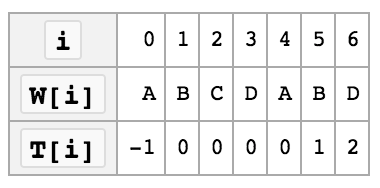
\includegraphics[scale=1.30]{kmp_table}}
\caption{Prefix-suffix table}
\label{fig:kmp_table}
\end{figure}
In table-building algorithm, similar to dp, let $T[i]$ store the length of matched prefix suffix for $needle[:i]$\\
\\
Clues:
\begin{enumerate}
\item dummy at $T[0]=-1$.
\item three parts
\begin{enumerate}
\item matched
\item fall back (consider $ABABC...ABABA$)
\item restart 
\end{enumerate}
\end{enumerate}
Table-building code:
\begin{python}
# construct T
T = [0 for _ in xrange(len(needle)+1)]
T[0] = -1
T[1] = 0

cnd = 0  
i = 2  # table index
while i < len(needle)+1:
    if needle[i-1] == needle[cnd]:  # matched
        T[i] = cnd+1
        cnd += 1
        i += 1
    elif T[cnd] != -1:  # fall back 
        cnd = T[cnd]
    else:  # restart 
        T[i] = 0
        cnd = 0
        i += 1
\end{python}
\subsection{Searching algorithm}
\begin{figure}[F]
\centering
\subfloat{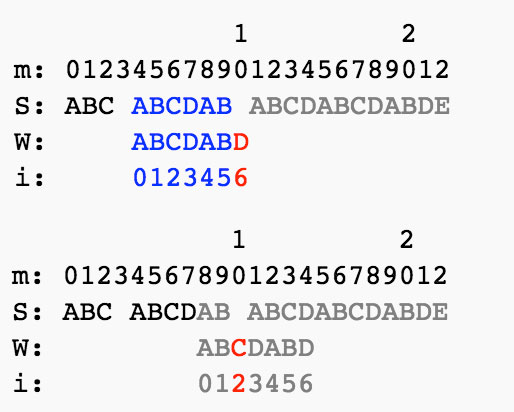
\includegraphics[scale=1.30]{kmp_presuffix}}
\caption{KMP example}
\label{fig:kmp_presuffix}
\end{figure}

Notice:
\begin{enumerate}
\item index $i$ and $j$.
\item $T[i-1+1]$ for corresponding previous index in $T$ for current scanning index $i$. 
\item When falling back, the next scanning index is \pyinline{len(prefix)}
\item three parts:
\begin{enumerate}
\item matched
\item aggressive move and fall back
\item restart 
\end{enumerate}
\end{enumerate}
Search code: 
\begin{python}
# search
i = 0  # index for needle 
j = 0  # index for haystack
while j+i < len(haystack):
    if needle[i] == haystack[j+i]:  # matched 
        i += 1
        if i == len(needle):
            return haystack[j:]
    else:
        if T[i] != -1:  # move and fall back j
            j = j+i-T[i]
            i = T[i]
        else:  # restart
            j += 1
            i = 0

return None
\end{python}
\subsection{Applications}
\begin{enumerate}
\item Find needle in haystack. 
\item Shortest palindrome 
\end{enumerate}


\chapter{Stream}
\section{Sliding Window}
\runinhead{Sliding Window Maximum.} Given an array $nums$, Find the list of maximum in the sliding window of size $k$ which is moving from the very left of the array to the very right. $\rightarrow$ double-ended queue.

Invariant: the queue is storing the non-decreasing-ordered elements of current window.

\runinhead{Sliding Window Median.} Find the list of median in the sliding window. $\rightarrow$ Dual heap with lazy deletion - section \ref{dh_lazy_del}.

\chapter{Math}

\section{Functions}
\rih{Equals.} Requirements for equals
\begin{enumerate}
\item Reflexive
\item Symmetric
\item Transitive
\item Non-null
\end{enumerate}
\rih{Compare.} Requirements for compares (total order):
\begin{enumerate}
\item Antisymmetry
\item Transitivity
\item Totality
\end{enumerate}

\section{Prime Numbers}
\subsection{Sieve of Eratosthenes}
\subsubsection{Basics}
To find all the prime numbers less than or equal to a given integer n by Eratosthenes' method:
\begin{enumerate}
\item Create a list of consecutive integers from 2 through n: (2, 3, 4, ..., n).
\item Initially, let $p$ equal 2, the first prime number.
\item Starting from $p$, enumerate its multiples by counting to n in increments of $p$, and mark them in the list (these will be $2p$, $3p$, $4p$, ... ; the $p$ itself should not be marked).
\item Find the first number greater than $p$ in the list that is not marked. If there was no such number, stop. Otherwise, let $p$ now equal this new number (which is the next prime), and repeat from step 3.
\end{enumerate}

When the algorithm terminates, the numbers remaining not marked in the list are all the primes below $n$.

\subsubsection{Refinements}
The main idea here is that every value for $p$ is prime, because we have already marked all the multiples of the numbers less than $p$. Note that some of the numbers being marked may have already been marked earlier (e.g., 15 will be marked both for 3 and 5).

As a refinement, it is sufficient to mark the numbers in step 3 starting from $p^2$, because all the smaller multiples of $p$ will have already been marked at that point by the previous smaller prime factor other than $p$. From $p^2$, $p$ becomes the smaller prime factor of a composite number. This means that the algorithm is allowed to terminate in step 4 when $p^2$ is greater than n.

Another refinement is to initially list odd numbers only, (3, 5, ..., n), and count in increments of $2p$ in step 3, thus marking only odd multiples of $p$. This actually appears in the original algorithm. This can be generalized with wheel factorization, forming the initial list only from numbers coprime with the first few primes and not just from odds (i.e., numbers coprime with 2), and counting in the correspondingly adjusted increments so that only such multiples of $p$ are generated that are coprime with those small primes, in the first place.

To summarized, the refinements include:
\begin{enumerate}
\item Starting from $p^2$.
\item Preprocessing even numbers and then only process odd numbers; thus the increment becomes $2p$.
\end{enumerate}}

\subsubsection{code}
\begin{python}
def countPrimes(n):
    """
    Find prime using Sieve's algorithm
    :type n: int
    :rtype: int
    """
    if n < 3:
        return 0

    is_prime = [True for _ in xrange(n)]
    is_prime[0], is_prime[1] = False, False
    for i in xrange(2, int(math.sqrt(n))+1):
        if is_prime[i]:
            for j in xrange(i*i, n, i):
                is_prime[j] = False

    return is_prime.count(True)
\end{python}

\subsection{Factorization}
Backtracking: Section-\ref{factorization}.

\section{Median}
\subsection{Basic DualHeap}
DualHeap to keep track the median when a method to find median is called multiple times. \begin{python}
import heapq

class DualHeap(object):
  def __init__(self):
    self.min_h = []
    self.max_h = []  # need to negate the value 

  def insert(self, num):
    if not self.min_h or num > self.min_h[0]:
      heapq.heappush(self.min_h, num)
    else:
      heapq.heappush(self.max_h, -num)
    self.balance()

  def balance(self):
    l1 = len(self.min_h)
    l2 = len(self.max_h)
    if l1-l2 > 1:
      heapq.heappush(self.max_h, 
                     -heapq.heappop(self.min_h))
      self.balance()
    elif l2-l1 > 1:
      heapq.heappush(self.min_h, 
                     -heapq.heappop(self.max_h))
      self.balance()
    return

  def get_median(self):
    """Straightforward"""
\end{python}

\subsection{DualHeap with Lazy Deletion}\label{dh_lazy_del}
Clues:
\begin{enumerate}
\item Wrap the value and wrap the heap
\item When delete a value, mark it with tombstone. 
\item When negate the value, only change the value, not the reference. 
\item When heap pop, clean the op first. 
\end{enumerate}
\begin{python}
import heapq
from collections import defaultdict


class Value(object):
    def __init__(self, val):
        self.val = val
        self.deleted = False

    def __neg__(self):
        """negate without creating new instance"""
        self.val = -self.val
        return self

    def __cmp__(self, other):
        assert isinstance(other, Value)
        return self.val - other.val

    def __repr__(self):
        return repr(self.val)


class Heap(object):
    def __init__(self):
        self.h = []
        self.len = 0

    def push(self, item):
        heapq.heappush(self.h, item)
        self.len += 1

    def pop(self):
        self._clean_top()
        self.len -= 1
        return heapq.heappop(self.h)

    def remove(self, item):
        """lazy delete"""
        item.deleted = True
        self.len -= 1

    def __len__(self):
        return self.len

    def _clean_top(self):
        while self.h and self.h[0].deleted:
            heapq.heappop(self.h)

    def peek(self):
        self._clean_top()
        return self.h[0]


class DualHeap(object):
    def __init__(self):
        self.min_h = Heap()  # represent right side
        self.max_h = Heap()  # represent left side
    # others similar as the previous section's above DualHeap
\end{python}

\chapter{Arithmetic}


\section{Big Number}
\rih{Plus One.} Given a non-negative number represented as an array of digits, plus one to the number.
\begin{python}
def plusOne(self, digits):
    for i in xrange(len(digits)-1, -1, -1):
        digits[i] += 1
        if digits[i] < 10:
            return digits
        else:
            digits[i] -= 10

    # if not return within the loop 
    digits.insert(0, 1)
    return digits
\end{python}

\section{Polish Notations}
Polish Notation is in-fix while Reverse Polish Notation is post-fix. 

Reverse Polish notation (RPN) is a mathematical notation in which every operator follows all of its operands (i.e. operands are followed by operators). RPN should be treated as the orthogonal expression.  

Polish notation (PN) is a mathematical notation in which every operator is followed by its operands. 

\subsection{Convert in-fix to post-fix (RPN)}
\pyinline{ret} stores the final result of reverse polish notation. \pyinline{stk} stores
the temporary result in strictly increasing order. 

In-fix
\begin{python}
5 + ((1 + 2) * 4) - 3
\end{python}

can be written as
\begin{python}
5 1 2 + 4 * + 3 - 
\end{python}
Core clues:
\begin{enumerate}
\item \rih{Stack}. The stack temporarily stores the operators of \textit{strictly increasing precedence order}.
\item \rih{Precedence}. Digits have the highest precedence, followed by \pyinline{*, /, +, (}. Notice that \pyinline{(} operator itself has the \textit{lowest} precedence.
\item \rih{Bracket}. \textit{Match} the brackets. 
\end{enumerate}
Code:
\begin{python}
def infix2postfix(self, lst):
  stk = []
  ret = []  # post fix result
  for elt in lst:
    if elt.isdigit():
      ret.append(elt)
    elif elt == "(":
      stk.append(elt)
    elif elt == ")":
      while stk and stk[-1] != "(":
        ret.append(stk.pop())
      stk.pop()  # pop "("
    else:
      while stk and precdn(elt) <= precdn(stk[-1]):
        ret.append(stk.pop())
      stk.append(elt)

  while stk:  # clean up 
    ret.append(stk.pop())

  return ret
\end{python}

\subsection{Evaluate post-fix expressions}\label{section:evaluationPostFix}
Consider: 

In-fix
\begin{python}
5 + ((1 + 2) * 4) - 3
\end{python}

Post-fix
\begin{python}
5 1 2 + 4 * + 3 - 
\end{python}
Straightforward: use a \textit{stack} to store the number. Iterate the input, push
stack when hit numbers, pop stack when hit operators.

\subsection{Convert in-fix to pre-fix (PN)}
PN is the \textit{reverse} of RPN, thus, scan the expression from right to left; and \pyinline{stk} stores the temporary result in non-decreasing order. 


In-fix
\begin{python}
5 + ((1 + 2) * 4) - 3
\end{python}

can be written as
\begin{python}
3 4 2 1 + * 5 + -
\end{python}

reverse as 
\begin{python}
- + 5 * + 1 2 4 3
\end{python}

\begin{python}
  def infix2prefix(self, lst):
    """starting from right the left"""
    stk = []
    pre = []
    for elt in reversed(lst):
      if elt.isdigit():
        pre.append(elt)
      elif elt == ")":
        stk.append(elt)
      elif elt == "(":
        while stk and stk[-1] != ")":
          pre.append(stk.pop())
        stk.pop()
      else:
        # < rather than <=
        while stk and precdn(elt) < precdn(stk[-1]):  
          pre.append(stk.pop())
        stk.append(elt)

    while stk:
      pre.append(stk.pop())

    pre.reverse()
    return pre
\end{python}


\subsection{Evaluate pre-fix (PN) expressions}
Consider: 

In-fix
\begin{python}
5 + ((1 + 2) * 4) - 3
\end{python}

Pre-fix
\begin{python}
- + 5 * + 1 2 4 3
\end{python}

reverse as 
\begin{python}
3 4 2 1 + * 5 + -
\end{python}
Put into \textit{stack}, similar to evaluating post-fix \ref{section:evaluationPostFix}, but pay attention to operands order, which should be reversed when hitting a operator. 

\chapter{Combinatorics}
\section{Basics}
\subsection{Considerations}
\begin{enumerate}
\item Does \textbf{order} matter?
\item Are the objects \textbf{repeatable}?
\item Are the objects partially \textbf{duplicated}?
\end{enumerate}}
If order does not matter, you can pre-set the order. 
\subsection{Basic formula}
\begin{eqnarray*}
&& {n \choose k} = \frac{n!}{k!(n-k)!} \\
&& {n \choose k} = {n \choose n-k} \\
&& {n\choose k} = {n-1\choose k} + {n-1 \choose k-1}
\end{eqnarray*}

\subsection{N objects, K ceils}
When $N=10, K=3$:
$$
x_1 + x_2 + x_3 = 10
$$
is equivalent to
$$
*****|**|***
$$

, notice that $*$ are non-order.
\\
then the formula is:
$$
{n+r \choose r}
$$

,where $r=k-1$. 
\\
The meaning is to choose $r$ objects from $n+r$ objects to become the $|$.

\subsection{N objects, K types} \label{N_objects_K_types}
What is the number of permutation of $N$ objects with $K$ different types:
\begin{align*}
ret &= \frac{A_N^N}{\prod_{k=1}^K{A_{sz(k)}^{sz(k)}}} \\
&= \frac{N!}{\prod_{k} sz[k]!}
\end{align*}

\subsection{Inclusion–Exclusion Principle}
\begin{figure}[hbtp]
\centering
\subfloat{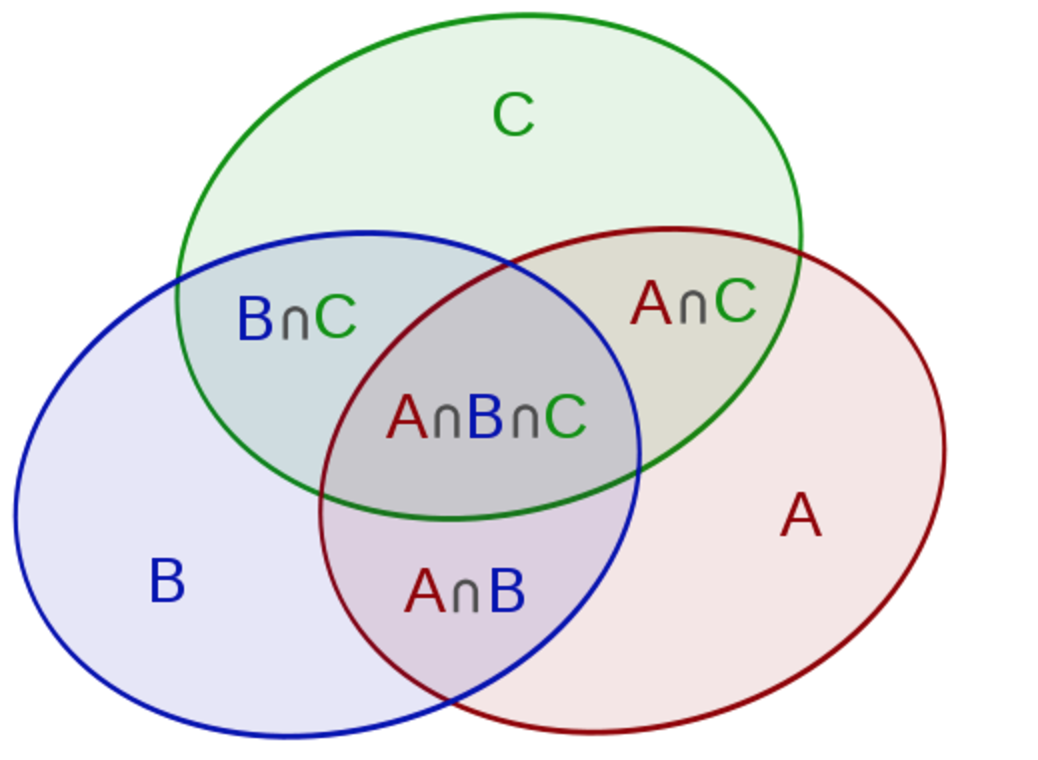
\includegraphics[scale=0.50]{500px-Inclusion-exclusion}}
\caption{Inclusion–exclusion principl}
\label{fig:500px-Inclusion-exclusion}
\end{figure}
\begin{eqnarray*}
|A \cup B \cup C| = |A| + |B| + |C| \\ - |A \cap B| - |A \cap C| - |B \cap C| \\ + |A \cap B \cap C|
\end{eqnarray*}
Generally,
$$
\Biggl|\bigcup_{i=1}^n A_i\Biggr| = \sum_{k = 1}^{n} (-1)^{k+1} \left( \sum_{1 \leq i_{1} < \cdots < i_{k} \leq n} \left| A_{i_{1}} \cap \cdots \cap A_{i_{k}} \right| \right)
$$
\section{Combinations with Duplicated Objects}
Determine the number of combinations of 10 letters (order does not matter) that can be formed from 3A, 4B, 5C. 

\subsection{Basic Solution}
If there are no restrictions on the number of any of the letter, it is ${10+2 \choose 2}$; then we get the universal set, 
$$
|U|={10+2 \choose 2}
$$

Let $P_A$ be the set that a 10-combination has more than 3A. $P_B$...4B. $P_C$...5C. 

The result is:
\begin{eqnarray*}
&& |3A \cap 4B \cap 5C| = \\
&& |U| - sum(|P_i|) + sum(|P_i \cap P_j|) - sum(|P_i \cap P_j \cap
P_k|)
\end{eqnarray*}

To calculate $|P_i|$, take $|P_1|$ as an example. \textbf{Pre-set} 4A -- if we take any one of these 10-combinations in $P_1$ and remove 4A we are left with a 6-combination with unlimited on the numbers of letters; thus,
$$
|P_1|={6+2 \choose 2}
$$

Similarly, we can get $P_2, P_3$.

To calculate $|P_i \cap P_j}|$, take $|P_1 \cap P_2|$ as an example. \textbf{Pre-set} 4A and 5B; thus,
$$
|P_1 \cap P_2| = {1+2 \choose 2}
$$

Similarly, we can get other $|P_i \cap P_j|$.

Similarly, we can get other $|P_i \cap P_j \cap P_k|$.
\subsection{Algebra Solution}
The number of 10-combinations that can be made from 3A, 4B, 5C is found from the coefficient of $x^{10}$ in the expansion of:
$$
(1+x+x^2+x^3)(1+x+x^2+x^3+x^4)(1+x+x^2+x^3+x^4+x^5)
$$

And we know:
\begin{eqnarray*}
1+x+x^2+x^3         = (1-x^4)/(1-x)  \\
1+x+x^2+x^3+x^4     = (1-x^5)/(1-x)  \\
1+x+x^2+x^3+x^4+x^5 = (1-x^6)/(1-x)  \\
\end{eqnarray*}


We expand the formula, although the  naive way of getting the coefficient of $x^{10}$ is tedious. 

\section{Permutation}

\subsection{$k$-th permutation}
Given $n$ and $k$, return the $k$-th permutation sequence. $k\in [1, n!]$. $O(nk)$ in time complexity is easy, can you do it in $O(n^2)$ or less?

Reversed Cantor Expansion

Core clues:
\begin{enumerate}
\item \pyinline{A = [1, 2, ..., n]}

Suppose for $n$ element, the $k$-th permutation is:

\pyinline{ret = [a0, a1, a2, ..., an-1]}
\item \rih{Basic case.} Since \pyinline{[a1, a3, ..., an-1]} has $(n-1)!$ permutations,
if $k < (n-1)!, a_0 = A_0$ (first element in array), else $a_0 = A_{k/(n-1)!}$

\item Recursively, (or iteratively), calculate the values at each position. Similar to Radix. 
\begin{enumerate}
\item $a_0 = A_{k_0/(n-1)!}$, where $k_0 = k$
\item $a_1 = A_{k_1/(n-2)!}$, where $k_1 = k_0\%(n-1)!$ in the remaining array $A$
\item $a_2 = A_{k_2/(n-3)!}$, where $k_2 = k_1\%(n-2)!$ in the remaining array $A$
\end{enumerate}
\end{enumerate}
\begin{python}
def getPermutation(self, n, k):
    k -= 1  # start from 0

    A = range(1, n+1)
    k %= math.factorial(n)
    ret = []
    for i in xrange(n-1, -1, -1):
        idx, k = divmod(k, math.factorial(i))
        ret.append(A.pop(idx))

    return "".join(map(str, ret))
\end{python}

\section{Catalan Number}\label{section:catalanNumber}
\subsection{Math}
\runinhead{Definition.}
$$
C_n = {2n\choose n} - {2n\choose n+1} = {1\over n+1}{2n\choose n} \quad\text{ for }n\ge 0
$$
\runinhead{Proof.} Proof of Calatan Number $C_n ={2n\choose n} - {2n\choose n+1}$. Objective: count the number of paths in $n\times n$ grid without exceeding the main diagonal. 
\begin{itemize}
\begin{figure}[]
    \centerline{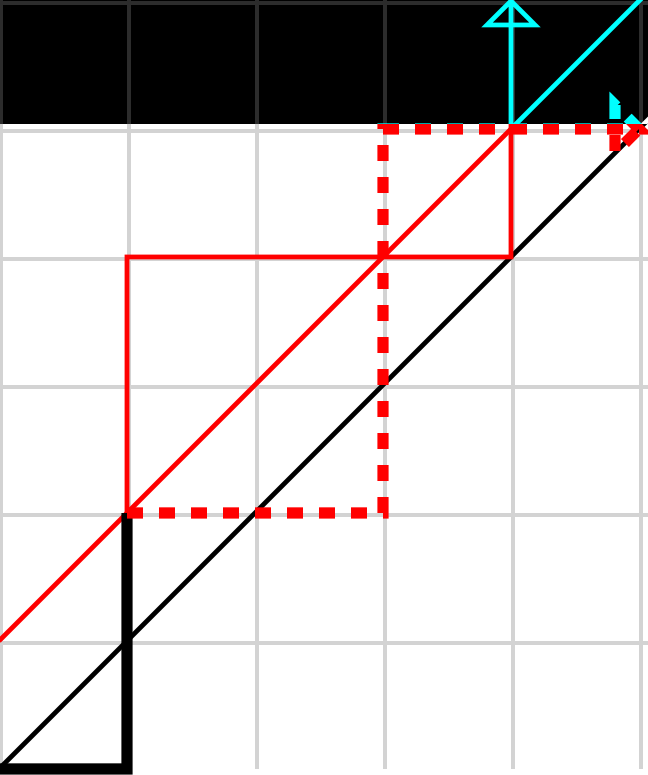
\includegraphics[height = 1.6in]{catalan_proof}}
    \caption{Monotonic Paths}
  \label{fig:catalanProof}
\end{figure}
\item monotonic paths - $n$ right, $n$ up
$$
{2n\choose n}
$$
\item flip at the line just above the diagonal line - $n-1$ right, $n+1$ up
$$
{n-1+n+1\choose n-1}
$$
\item thus, the number of path without \textit{exceedance} (i.e. passing the diagonal line) is: 
\begin{align*}
C_n &= {2n\choose n} - {2n\choose n-1}\\ 
&={2n\choose n} - {2n\choose n+1}
\end{align*}
\end{itemize}

\subsection{Applications}
The paths in Figure \ref{fig:catalanProof} can be abstracted to anything that at any time \#right $\geq$ \#up. 
\runinhead{\#Parentheses.}Number of different ways of adding parentheses. At any time, \#\pyinline{(} $\geq$ \#\pyinline{)}.
\runinhead{\#BSTs.}Number of different BSTs. Consider it as a set of same binary operators with their operands. Reduce this problem to \#Parentheses. 
\begin{figure}[hbtp]
\centering
\subfloat{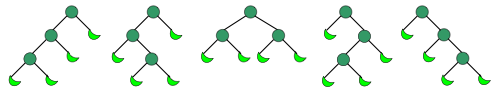
\includegraphics[scale=2.00]{Catalan_number_binary_tree_example}}
\caption{\#BSTs. Circles are operators; crescents are operands.}
\label{fig:NumberOfBSTs}
\end{figure}

\section{Stirling Number}
a Stirling number of the second kind (or Stirling partition number) is the number of ways to partition a set of n objects into k non-empty subsets and is denoted by $S(n,k)$ or  $\lbrace{n\atop k}\rbrace$.

$$
\left\{ {n \atop k}\right\} = \frac{1}{k!}\sum_{j=0}^{k} (-1)^{k-j} \binom{k}{j} j^n.
$$

\chapter{Probability}


\section{Shuffle}
Equal probability shuffle algorithm.

\subsection{Incorrect naive solution}
Swap current card $A_i$ with a random card from the deck. 
\begin{java}
for (int i = 0; i < N; i++) {
   int j = (int) Math.random()*N;
   swap(a[i], a[j]);
}
\end{java}
The easiest proof that this algorithm does not produce a uniformly random permutation is that it generates 27 possible outcomes, but there are only 3! = 6 permutations. Since $27\%3 \neq 0$, there must be some permutation is that is picked too much, and some that is picked to little.
\subsection{Knuth Shuffle}
Knuth (aka Fisher-Yates) shuffling algorithm guarantees to rearrange the elements in uniformly random order. 
\\
Core clues:
\begin{enumerate}
\item choose index uniformly $\in [i, N)$
\end{enumerate}
\begin{java}
public void shuffle(Object[] a) {
    int N = a.length;
    for (int i = 0; i < N; i++) {
        // choose index uniformly in [i, N)
        int j = i + (int) (Math.random() * (N - i));
        swap(a[i], a[j]);
    }
}
\end{java}

\section{Expected Value}
\subsection{Roll dice until expected value.}


\chapter{Bit Manipulation}
\section{Concepts}
\subsection{Basics}
\begin{enumerate}
\item Bit value: bit0, bit1. 
\item BitSet/Bits
\item Bit position (bit interchangeably)
\item 32-bit signed range: $[-2^{31}, 2^{31}-1]$. $0$ is like positive number without complement. 
\end{enumerate}
\subsection{Operations}
\runinhead{Mask.} 
\begin{enumerate}
\item Masking to 1: to mask a single bit position, $bit\OR 1$
\item Masking to 0: to mask a single bit position, $bit\AND 0$
\item Querying a bit position value: to query a single bit position, $bit\AND 0010$
\item Toggling bit values: to toggle a single bit position, $bit\XOR 1$
\end{enumerate}}
This can be extended to do masking operations on multiple bits. 

\runinhead{Check 2's power}
$$x\AND(x-1)$$

\runinhead{Rightmost bit set.} To get the rightmost bit, with the help of 2's complement:
\begin{enumerate}
\item Left extended with 1's:
$$x \XOR (-x)$$
\item Left extended with 0's:
$$x \AND (-x)$$
\end{enumerate}

\runinhead{Negation and index} We can use tilde notation for the index accessing a string or an array
\begin{lstlisting}
i  ~i  
0  -1
1  -2
2  -3
3  -4 
4  -5 
5  -6
\end{lstlisting}
$$
\NOT i = -i+1
$$
To determine whether a string is palindrome:
\begin{python}
def is_palindrome(s):
  return all(s[i] == s[~i] for i in xrange(len(s)/2)) 
\end{python}
\section{Single Number}
\subsection{Three-time appearance} 
Given an array of integers, every element appears three times except for one. Find that single one.

\rih{Using list.} Consider 4-bit numbers:
\begin{eqnarray*}
&& 0000 \\
&& 0001 \\
&& 0010 \\
&& ... \\
&& 1111
\end{eqnarray*}

Add (not $\&$) the bit values \textbf{vertically}, then result would be $abcd$ where $a, b, c, d$ can be any number, not just binary. $a, b, c, d$ can be divided by 3 if the all element appears three times. Until here, you can use a list to hold $a, b, c, d$. By mod 3, the single one that does not appear 3 times is found. 

To generalize to 32-bit \pythoninline{int}, use a list of length 32.

\rih{Using bits.}
To further optimize the space, use bits (bit set) instead of list. 
\begin{itemize}
\item Since all except one appears 3 times, we are only interested in $0, 1, 2$ (mod 3) count of bit1 appearances in a bit position.
\item We create 3 bit sets to represent $0, 1, 2$ appearances of all positions of bits.
\item For a bit, there is one and only one bit set containing bit1 in that bit position.
\item Transition among the 3 bit sets for every number:
$$
bitSet^{(i)} = (bitSet^{(i-1)}\AND num)\OR(bitSet^{(i)}\AND \NOT num)
$$
\end{itemize}

For $i$ appearances, the first part is the bit set \textbf{transited from} $(i-1)$ appearances, and the second part is the bit set \textbf{transited out} from itself.

Consider each single bit separately. For the $j$-th bit in $num$, if $num_j=1$, the first part indicates $bitSet^{(i-1)}$ will transit in (since transition); the 2nd part is always 0 (since transition out or initially 0). If $num_j=0$, the 1st part is always 0 (since no transition); the 2nd part indicates $bitSet^{(i)}$ will remain the same (since no transition). 



\subsection{Two Numbers} 
Given an array of numbers nums, in which exactly two elements appear only once and all the other elements appear exactly twice. Find the two elements that appear only once.

\begin{itemize}
\item Easily get: $x = a \XOR b$.
\item $a \neq b$; thus there are at least one 1-bit in $x$ is different.  
\item Take an arbitrary 1 bit set in $x$, and such bit set can classify the elements in the array into two separate groups.
\end{itemize}

\section{Bitwise operators}
\runinhead{Comparison.} Write a method which finds the maximum of two numbers $a, b$. You should not use if- else or any other comparison operator
\\
Clues:
\begin{enumerate}
\item check the sign bit $s$ of $a-b$.
\item return $a-s*(a-b)$
\end{enumerate}
Codes:
\begin{java}
int getMax(int a, int b) { 
    int c = a - b;
    int k = (c >> 31) & 0x1; 
    int max = a - k * c; 
    return max;
}

\end{java}
If consider overflow, it raises another level of difficulty. 

\chapter{Greedy}

\section{Introduction}
Philosophy: choose the best options at the current state without reverting the choice in the future. 

A greedy algorithm is an algorithm that follows the problem solving heuristic of making the locally optimal choice at each stage with the hope of finding a global optimum.

\chapter{Backtracking}
\section{Introduction}
\runinhead{Difference between backtracking and dfs.} \textit{Backtracking} is a more general purpose algorithm. \textit{Dfs} is a specific form of backtracking related to searching tree structures. 

\runinhead{Prune.} Backtrack need to think about pruning using the condition \pyinline{predicate}.

\section{Sequence}
\runinhead{k sum.} Given $n$ unique integers, number $k$ and target. Find all possible $k$ integers where their sum is target. 

Complexity: $O(2^n)$.

Pay attention to the pruning condition.

\begin{python}
def dfs(self, A, i, k, cur, remain, ret):
    """self.dfs(A, 0, k, [], target, ret)"""
    if len(cur) == k and remain == 0:
        ret.append(list(cur))
        return

    if (i >= len(A) or len(cur) > k 
        or len(A)-i+len(cur) < k):
        return

    self.dfs(A, i+1, k, cur, remain, ret)
    cur.append(A[i])
    self.dfs(A, i+1, k, cur, remain-A[i], ret)
    cur.pop()
\end{python}


\section{String}
\subsection{Palindrome}
\subsubsection{Palindrome partition.} Given \pyinline{s = "aab"}, return: \\
\pyinline{[["aa","b"], ["a","a","b"]]}
\\
\runinhead{Core clues:}
\begin{enumerate}
\item Expand the search tree \textbf{horizontally}.
\end{enumerate}
\rih{Search process:}
\begin{python}
input: "aabbc"

"a", "abbc"
     "a", "bbc"
          "b", "bc"
               "b", "c" (o)
               "bc" (x)
          "bb", "c" (o)
          "bbc" (x)
     "ab", "bc" (x)
     "abb", "c" (x)
     "abbc" (x)
"aa", "bbc"
      "b", "bc"
           "b", "c" (o)
           "bc" (x)
      "bb", "c" (o)
      "bbc" (x)
"aab", "bc" (x)
"aabb", "c" (x)
\end{python}
Code:

\begin{python}
def partition(self, s):
    ret = []
    self.backtrack(s, [], ret)
    return ret

def backtrack(self, s, cur_lvl, ret):
    """
    Let i be the scanning ptr.
    If s[:i] passes predicate, then backtrack s[i:]
    """
    if not s:
        ret.append(list(cur_lvl))

    for i in xrange(1, len(s)+1):
        if self.predicate(s[:i]):
            cur_lvl.append(s[:i])
            self.backtrack(s[i:], cur_lvl, ret)
            cur_lvl.pop()

def predicate(self, s):
    return s == s[::-1]
\end{python}



\section{Math}
\subsection{Decomposition}
\subsubsection{Factorize a number}\label{factorization}
\runinhead{Core clues:}
\begin{enumerate}
\item Expand the search tree \textbf{horizontally}.
\end{enumerate}
\runinhead{Search tree:}
\begin{python}
Input: 16
get factors of cur[-1]
[16]
[2, 8]
[2, 2, 4]
[2, 2, 2, 2]

[4, 4]
\end{python}
Code:
\begin{python}
def dfs(self, cur, ret):
  if len(cur) > 1:
    ret.append(list(cur))

  n = cur.pop()
  start = cur[-1] if cur else 2
  for i in xrange(start, int(sqrt(n))+1):
    if self.predicate(n, i):
      cur.append(i)
      cur.append(n/i)
      self.dfs(cur, ret)
      cur.pop()
            
def predicate(self, n, i):
  return n%i == 0
  
\end{python}
\runinhead{Time complexity.} The search tree's size is $O(2^n)$ where $n$ is the number
of prime factors. Choose $i$ prime factors to combine then, and keep the rest uncombined:


$$\sum_i {n \choose i} = 2^n$$


\section{Arithmetic Expression}
\subsection{Unidirection}
\rih{Insert operators.} Given a string that contains only digits 0-9 and a target value,
return all possibilities to add binary operators (not unary) +, -, or * between the
digits so they evaluate to the target value.

Example: 
\begin{align*}
``123", 6 \rightarrow [``1+2+3", ``1*2*3"] \\ 
``232", 8 \rightarrow [``2*3+2", ``2+3*2"] \\
\end{align*}
Clues:
\begin{enumerate}
\item Backtracking with \textit{horizontal} expanding
\item Special handling for multiplication - caching the expression \textit{predecessor}
for multiplication association. 
\item Detect \textit{invalid} number with leading 0's
\end{enumerate}

\begin{python}
def addOperators(self, num, target):
  ret = []
  self.dfs(num, target, 0, "", 0, 0, ret)
  return ret

def dfs(self, num, target, pos, 
        cur_str, cur_val, 
        mul, ret
):
  if pos >= len(num):
    if cur_val == target:
      ret.append(cur_str)
  else:
    for i in xrange(pos, len(num)):
      if i != pos and num[pos] == '0':
        continue
        
      nxt_val = int(num[pos:i+1])
      if not cur_str:  # 1st number
        self.dfs(num, target, i+1, 
            "%d"%nxt_val, nxt_val,
            nxt_val, ret)
      else:  # +, -, *
        self.dfs(num, target, i+1, 
            cur_str+"+%d"%nxt_val, cur_val+nxt_val, 
            nxt_val, ret)
        self.dfs(num, target, i+1, 
            cur_str+"-%d"%nxt_val, cur_val-nxt_val, 
            -nxt_val, ret)
        self.dfs(num, target, i+1, 
    cur_str+"*%d"%nxt_val, cur_val-mul+mul*nxt_val, 
            mul*nxt_val, ret)
\end{python}
\subsection{Bidirection}
\rih{Insert parenthesis.} Given a string of numbers and operators, return all possible
results from computing all the different possible ways to group numbers and operators.
The valid operators are +, - and *.

Examples:
\begin{align*}
(2*(3-(4*5))) &= -34 \\
((2*3)-(4*5)) &= -14 \\
((2*(3-4))*5) &= -10 \\
(2*((3-4)*5)) &= -10 \\
(((2*3)-4)*5) &= 10
\end{align*}
Clues: Iterate the operators, divide and conquer - left parts and right parts and then
combine result. \\
Code:
\begin{python}
def dfs_eval(self, nums, ops):
  ret = []
  if not ops:
    assert len(nums) == 1
    return nums

  for i, op in enumerate(ops):
    left_vals = self.dfs_eval(nums[:i+1], ops[:i])
    right_vals = self.dfs_eval(nums[i+1:], ops[i+1:])
    for l in left_vals:
      for r in right_vals:
        ret.append(self._eval(l, r, op))

  return ret
\end{python}
\section{Tree}
\subsection{BST}
\subsubsection{Generate Valid BST}
Generate all valid BST with nodes from 1 to $n$.
\runinhead{Core clues:}
\begin{enumerate}
\item Iterate pivot
\item Generate left and right
\end{enumerate}
Code:
\begin{python}
def generate(self, start, end):
  roots = []
  if start > end:
    roots.append(None)
    return roots

  for pivot in range(start, end+1):
    left_roots = self.generate_cache(start, pivot-1)
    right_roots = self.generate_cache(pivot+1, end)
    
    for left_root in left_roots:
      for right_root in right_roots:
        root = TreeNode(pivot)
        root.left = left_root
        root.right = right_root

        roots.append(root)

  return roots 

\end{python}



\chapter{Graph}

\section{Basic}
\runinhead{Graph representation.} $V$ for a vertex set with a map, mapping from vertex to its neighbors. The mapping relationship represents the edges $E$.
\begin{python}
V = defaultdict(list)
\end{python}

\runinhead{Complexity.} Basic complexities: 

\begin{tabular}{lll}
\hline\noalign{\smallskip}
\textbf{Algorithm} & \textbf{Time}  & \textbf{Space}\\
\noalign{\smallskip}\hline\noalign{\smallskip}
dfs & $O(|E|)$ & $O(|V|), O(\text{longest path})$ \\
bfs & $O(|E|)$ & $O(|V|)$ \\
\noalign{\smallskip}\hline\noalign{\smallskip}
\caption{CAPTIONS}
\end{tabular}

\section{DFS}
\rih{Number of Islands.} The most fundamental and classical problem. 
\begin{python}
11000
11000
00100
00011
Answer: 3
\end{python}
\rih{Clue}:
\begin{enumerate}
\item Iterative dfs
\end{enumerate}
\begin{python}
class Solution(object):
  def __init__(self):
    self.dirs = [(-1, 0), (1, 0), (0, -1), (0, 1)]

  def numIslands(self, grid):
    cnt = 0
    visited = [[False for _ in xrange(n)] 
               for _ in xrange(m)]
    for i in xrange(m):
      for j in xrange(n):
        if not visited[i][j] and grid[i][j] == "1":
          self.dfs(grid, i, j, visited)
          cnt += 1

    return cnt
\end{python}
\newpage
\begin{python}
  def dfs(self, grid, i, j, visited):
    m = len(grid)
    n = len(grid[0])
    visited[i][j] = True

    for dir in self.dirs:
      I = i+dir[0]
      J = j+dir[1]
      if (0 <= I < m and 0 <= J < n and 
        not visited[I][J] and grid[I][J] == "1"):
        self.dfs(grid, I, J, visited)
\end{python}
If the islands are constantly updating and the query for number of islands is called multiple times, need to use union-find (Section \ref{section:unionFind}) to reduce each query's complexity from $O(mn)$ to $O(\log mn)$.

\section{BFS}
\subsection{BFS with Abstract Level}
Start bfs with a set of vertices in abstract level, not necessarily neighboring vertices.

Example: $-1$ obstacles, $0$ targets, calculate all other vertices' Manhattan distance to its nearest target:
$$
\begin{bmatrix}
\infty & -1 & 0 & \infty \\
\infty & \infty & \infty & -1 \\
\infty & -1 & \infty & -1 \\
0 & -1 & \infty & \infty \\
\end{bmatrix} 
$$

is calculated as:
$$
\begin{bmatrix}
3 & -1 & 0 & 1 \\
2 & 2 & 1 & -1 \\
1 & -1 & 2 & -1 \\
0 & -1 & 3 & 4 \\
\end{bmatrix}
$$
\newpage
\rih{Code:}
\begin{python}
self.dirs = ((-1, 0), (1, 0), (0, -1), (0, 1))

def wallsAndGates(self, mat):
  q = [(i, j) for i, row in enumerate(mat) 
     for j, val in enumerate(row) if val == 0]
  for i, j in q:  # iterator
    for d in self.dirs:
      I, J = i+d[0], j+d[1]
      if (0 <= I < m and  0 <= J < n and 
        mat[I][J] > mat[i][j]+1):
        mat[I][J] = mat[i][j]+1
        q.append((I, J))
\end{python}


\section{Detect Acyclic}
\begin{enumerate}
\item \pythoninline{marked} is reset after a dfs. 
\item \pythoninline{visited} should be updated only in the end of the dfs. 
\item For directed graph:
\begin{enumerate}
\item Should dfs for all neighbors except for vertices in \pythoninline{visited}, to avoid revisiting. For example, avoid revisiting A, B when start from C in the graph $C \rightarrow A \rightarrow B$.
\item Excluding predecessor \pythoninline{pi} is erroneous in the case of $A \leftrightarrow B$ 
\end{enumerate}
\item For undirected graph:
\begin{enumerate}
\item Should dfs for all neighbors except for the predecessor \pythoninline{pi}. $A-B$.
\item Excluding neighbors in \pythoninline{visited} is redundant, due to \pyinline{pi}. 
\end{enumerate}
\end{enumerate}

\subsection{Directed Graph}
Detect cycles (any) in directed graph.

\begin{python}
def dfs(self, V, v, visited, pathset):
  if v in pathset:
    return False

  pathset.add(v)
  for nbr in V[v]:
    if nbr not in visited:
      if not self.dfs(V, nbr, visited, pathset):
        return False

  pathset.remove(v)
  visited.add(v)
  return True
\end{python}


\subsection{Undirected Graph}
Detect cycles (any) in undirected graph.

\begin{python}
def dfs(self, V, v, pi, visited, pathset):
  if v in pathset:
    return False

  pathset.add(v)
  for nbr in V[v]:
    if nbr != pi:
      if not self.dfs(V, nbr, v, visited, pathset):
        return False

  pathset.remove(v)
  visited.add(v)
  return True
\end{python}

\section{Topological Sorting}
For a graph $G=\{V, E\}$, if $A \rightarrow B $, then $A$ is before $B$ in the ordered list. 
\subsection{Algorithm}
\rih{Core clues}:
\begin{enumerate}
\item \textbf{Dfs neighbors first}. If the neighbors of current node is  $\neg$visited, then dfs the neighbors
\item \textbf{Process current node}. After visiting all the neighbors, then visit the current node and push it to the result queue.

\end{enumerate}
Notice:
\begin{enumerate}
\item Need to check ascending order or descending order. 
\item Need to \textbf{detect cycle}; thus the dfs need to construct result queue and detect cycle simultaneously, by using two sets: $visited$ and $pathset$. 
\end{enumerate}
\newpage
\begin{python}
from collections import deque

def topological_sort(self, V):
  visited = set()
  ret = deque()

  for v in V.keys():
    if v not in visited:
      if not self.dfs_topo(V, v, visited, set(), ret):
        return []  # contains cycle 

  return list(ret)

def dfs_topo(self, V, v, visited, pathset, ret):
  if v in pathset:
    return False

  pathset.add(v)
  for nbr in V[v]:
    if nbr not in visited:
      if not self.dfs_topo(V, nbr, visited, pathset, ret):
        return False

  pathset.remove(v)
  visited.add(v)
  ret.appendleft(v)
  return True

\end{python}

\subsection{Applications}
\begin{enumerate}
\item Course scheduling problem with pre-requisite. 
\end{enumerate}

\section{Union-Find}\label{section:unionFind}
Improvements:
\begin{enumerate}
\item Weighting: size-baladnced tree
\item Path Compression. 
\end{enumerate}}
\subsection{Algorithm}
Weighted union-find with path compression.\\
\rih{Core clues.} 
\begin{enumerate}
\item \textbf{$\pi$ array}:an array to store each item's predecessor pi. The predecessor are lazily updated to its ancestor. When \pyinline{x == pi[x]}, then \pyinline{x} is the ancestor (i.e. root).
\item \textbf{Size-balanced}: merge the tree according to the size to maintain balance.
\item \textbf{Path compression}: Make the ptr in $\pi$ array to point to its root rather than its immediate parent. 
\end{enumerate}
\begin{figure}[]
\centering
\subfloat{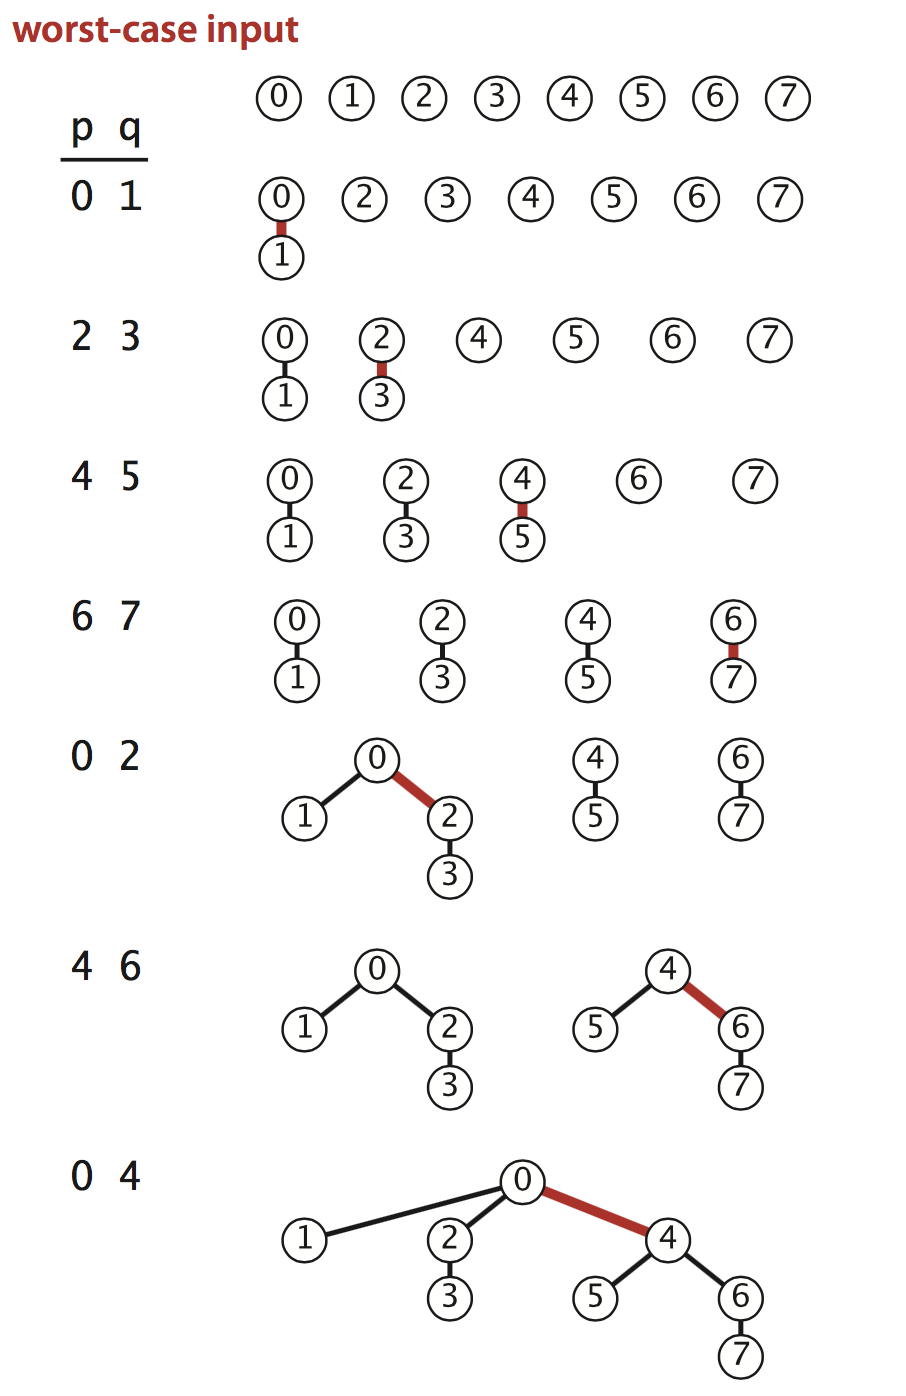
\includegraphics[scale=.70]{uf}}
\caption{Weighted quick-union traces}
\label{fig:union_find}
\end{figure}

\newpage
\begin{python}
class UnionFind(object):
  def __init__(self):
    self.pi = {}  # item -> pi
    self.sz = {}  # root -> size

  def __len__(self):
    """number of unions"""
    return len(self.sz)  # only root nodes have size

  def add(self, x):
    if x not in self.pi:
      self.pi[x] = x
      self.sz[x] = 1

  def root(self, x):
    """path compression"""
    pi = self.pi[x]
    if x != pi:
      self.pi[x] = self.root(pi)
    return self.pi[x]

  def unionize(self, x, y):
    pi1 = self.root(x)
    pi2 = self.root(y)

    if pi1 != pi2:
      if self.sz[pi1] > self.sz[pi2]:
        pi1, pi2 = pi2, pi1
        # size balancing
      self.pi[pi1] = pi2
      self.sz[pi2] += self.sz[pi1]
      del self.sz[pi1]
    
  def isunion(self, x, y):
    if x not in self.pi or y not in self.pi:
      return False 
    return self.root(x) == self.root(y)
\end{python}

\subsection{Complexity}
$m$ union-find with $n$ objects: $O(n)+m O(\lg n)$


\section{Axis Projection}
Project the mat dimension from 2D to 1D, using \textit{orthogonal axis}.

\runinhead{Smallest bounding box.} Given the location $(x, y)$ of one of the 1's, return the area of the smallest bounding box that encloses 1's.
$$
\begin{bmatrix}
0& 0& 1& 0 \\
0& 1& 1& 0 \\ 
0& 1& 0& 0 \\
\end{bmatrix}
$$

Clues:
\begin{enumerate}
\item Project the 1's onto x-axis, binary search for the left bound and right bound of the bounding box. 
\item Do the same for y-axis. 
\end{enumerate}

Time complexity: $O(m\log n + n \log m)$, where $O(m), O(n)$ is for projection complexity. 

\chapter{Dynamic Programming}



\section{Introduction}
The core philosophy of dp:
\begin{enumerate}
\item The definition of \textbf{states} 
\item The definition of the \textbf{transition functions} among states 
\end{enumerate} 

The so called concept dp as memoization of recursion does not grasp the core philosophy of dp. 

The formula in the following section are unimportant. Instead, what is important is the definition of dp array and transition function derivation.
\subsection{Common practice}
\runinhead{Dummy.} Use dummies to avoid using if-else conditional branch.
\begin{enumerate}
\item Use $n+1$ dp arrays to reserve space for dummies. 
\item Iteration range is $[1, n+1)$.
\item $n+k$ for k dummies  
\end{enumerate}
\runinhead{State definition.} Two general sets of state definitions - the state 
\begin{enumerate}
\item ends \textit{at} index $i$
\item ends \textit{before} index $i$
\item ends \textit{at} or \textit{before} index $i$
\end{enumerate}

\runinhead{Space optimization.} To avoid MLE, we need to carry out space optimization. Let $o$ be other subscripts, $f$ be the transition function. 

Firstly,
$$
F_{i, o} = f\big(F_{i-1, o'}\big)
$$

should be reduced to 
$$
F_{o} = f\big(F_{o'}\big)
$$

Secondly,
$$
F_{i, o} = f\big(F_{i-1, o'}, F_{i-2. o'}\big)
$$

should be reduced to 
$$
F_{i, o} = f\big(F_{(i-1)\%2, o'}, F_{(i-2)\%2. o'}\big)
$$

More generally, we can be $(i-b)\%a$ to reduce the space down to $a$.

Notice:
\begin{enumerate}
\item Must iterate $o$ \textbf{backward} to un-updated value. 
\end{enumerate}



\section{Sequence}\label{dpSequence}

\subsection{Single-state dp}
\runinhead{Longest common subsequence.} Let $F_{i, j}$ be the LCS at string $a[:i]$ and $b[:j]$. We have two situations: $a[i]==b[j]$ or not.
\begin{eqnarray*}
F_{i. j} = \left\{ \begin{array}{rl}
  F_{i-1, j-1}+1 &\mbox{// if $a[i]==b[j]$} \\
  \max\Big(F_{i-1, j},&\mbox{// otherwise} \\
  F_{i,j-1}\Big)
       \end{array} \right.
\end{eqnarray*}


\runinhead{Longest common substring.} Let $F_{i, j}$ be the LCS at string $a[:i]$ and
$b[:j]$. We have two situations: $a[i]==b[j]$ or not.
\begin{eqnarray*}
F_{i. j} = \left\{ \begin{array}{rl}
  F_{i-1, j-1}+1 &\mbox{// if $a[i]==b[j]$} \\
  0 &\mbox{// otherwise}
       \end{array} \right.
\end{eqnarray*}

Because it is not necessary that $F_{i,j}\geq F_{i',j'}, \forall i,j\cdot i>i', j>j'$, the $gmax=max\big(\{{F_{i,j}\}\big)$.
\runinhead{Longest increasing subsequence}. Find the longest increasing subsequence of an array $A$.

let $F_i$ be the LIS length ends at $A_i$. 
\begin{eqnarray*}
F_i = \max(F[j]+1 \cdot\forall j < i) \text{ // if $A_i>A_j$}
\end{eqnarray*}

Then the global $maxa$ is:
$$
maxa = \max(F_i\cdot \forall i)
$$

Time complexity: $O(n^2)$

In code, notice the \pyinline{else}.
\begin{python}
F[i] = max(
    F[j] + 1 if A[i] > A[j] else 1
    for j in xrange(i)
)
\end{python}

Alternative solution using binary search in $O(n \log n)$ - Section \ref{extremeValueProblem}.

\runinhead{Maximum subarray sum.} Find the maximum subarray sum of $A$. 

Let $F_i$  be the maximum subarray sum ending at $A_{i}$
$$
F_i = \max(F_{i-1}+A_{i}, 0)
$$

Then the global $maxa$ is:
$$
maxa = \max(F_i\cdot \forall i)
$$


\runinhead{Maximum sum of non-adjacent cells.} Get the maximum sum of non-adjacent
cells of an array $A$.

Let $F_i$ be the maximum sum of non-adjacent cells for $A[:i]$. You have tow options:
choose $A_{i-1}$ or not.
\begin{align*}
F_{i} = \max\big(F_{i-1}, F_{i-2}+A_{i-1}\big)
\end{align*}
\runinhead{Edit distance} Find the minimum number of steps required to convert words $A$ to $B$ using inserting, deleting, replacing. 

Let $F_{i, j}$ be the minimum number
of steps required to convert $A[:i]$ to $B[:j]$.
\begin{eqnarray*}
F_{i, j} = \left\{ \begin{array}{rl}
  F_{i-1, j-1} &\mbox{// if $a[i]==b[j]$} \\
  \min\Big(F_{i, j-1}+1, &\mbox{// otherwise, insert}\\
  F_{i-1, j}+1, &\mbox{// delete}\\
  F_{i-1, j-1}+1\Big) &\mbox{// replace}\\
       \end{array} \right.
\end{eqnarray*}

\runinhead{Maximal square.} Find the largest rectangle in the matrix:
\begin{lstlisting}
1 0 1 0 0
1 0 1 1 1
1 1 1 1 1
1 0 0 1 0
\end{lstlisting}
Let $F_{i, j}$ represents the max square's length ended at $mat_{i, j}$ (lower right corner).
\begin{eqnarray*}
F_{i, j} = \left\{ \begin{array}{rl}
  \min\big(F_{i-1, j-1}, F_{i-1, j}, F_{i, j-1}\big)+1 &\mbox{// if $mat_{i, j}==1$} \\
  0 &\mbox{// otherwise}
       \end{array} \right.
\end{eqnarray*}

\subsection{Dual-state dp}
\runinhead{Maximal product subarray.} Find the subarray within an array $A$ which has the largest product. 
\begin{itemize}
\item Let $small_i$ be the smallest product end with $A_i$. 
\item Let $large_i$ be the largest product end with $A_i$.
\item The states can be negative. 
\end{itemize}
\begin{eqnarray*}
&& small_i = \min\big( A_i,\ small_{i-1}\cdot A_i,\ large_{i-1}\cdot A_i \big)
\nonumber \\
&& large_i = \max\big( A_i,\ small_{i-1}\cdot A_i,\ large_{i-1}\cdot A_i \big)
\end{eqnarray*}

It can be optimized to use space $O(1)$. 

\runinhead{Trapping Rain Water}
Given n non-negative integers representing an elevation map where the width of each
bar is 1, compute how much water it is able to trap after raining.
\begin{figure}[]
    \centerline{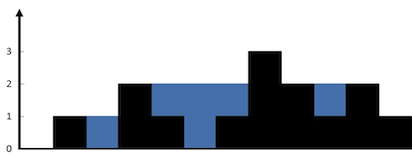
\includegraphics[height = 1in]{rainwatertrap}}
    \caption{Trapping Rain Water}
  \label{fig:rainwatertrap}
\end{figure}

Let $maxL_i$ be the $\max(A[:i])$; let $maxR_i$ be the $\max(A[i:n])$. The dp of obtaining max is trivial. 

The the total volume $vol$:
$$
vol = \sum_i(\max\big(0,\min(maxL_i, maxR_{i+1})-A[i]\big))
$$
\runinhead{Zigzag subsequence.} Find the max length zigzag subsequence which goes up and down alternately within the array $A$.

Let $U_i$ be the max length of zigzag subsequence end at $A_i \wedge$ going up.

Let $D_i$ be the max length of zigzag subsequence end at $A_i \wedge$ going down.
\begin{align*}
U_i &= max(D_j+1 \cdot \forall j < i) \text{ // if $A_i > A_j$} \\ 
D_i &= max(U_j+1 \cdot \forall j < i) \text{ // if $A_i < A_j$} 
\end{align*}

Notice in python implementation, don't use list comprehension since two states are interleaved and interdependent. 

\section{String}
\runinhead{Word break.} Given a string $s$ and a dictionary of words $dict$, determine if $s$ can be segmented into a space-separated sequence of $dict$ words.

Let $F_i$ be whether \pyinline{s[:i]} can be segmented. 
\begin{eqnarray*}
F_{i} = \left\{ \begin{array}{rl}
  F_{i-len(w)} &\mbox{// if $\exists w\in dict$, \pyinline{s[i-len(w):i]==w}}
\\
  false &\mbox{// otherwise}
       \end{array} \right.
\end{eqnarray*}
Return all such possible sentences. In original case, we use a bool array to record whether a dp could be segmented. Now we should use a vector for every dp to record how to construct that dp from another dp.

Let $F_i$ be all possible segmented words ends at \pyinline{s[i-1]}. $F_i$ is a list. $\exists F_i$ means $F_i$ is not empty.
\begin{eqnarray*}
F_{i} = \left\{ \begin{array}{rl}
  F_{i}+[w] &\mbox{// $\forall w\in dict\cdot$} \\
  & \mbox{ if \pyinline{s[i-len(w):i]==w} $\wedge\ \exists
F_{i-len(w)$ } \\
  F_{i}} &\mbox{// otherwise}
       \end{array} \right.
\end{eqnarray*}

Reconstruct the sentence from $F_i$. It is like building path for the tree. Using backtracking: 
\begin{python}
def build(self, dp, i, cur, ret):
    if cur_index == 0:
        ret.append(" ".join(list(cur)))
        return

    # backtracking
    for word in dp[i]:
        cur.appendleft(word)
        self.build(dp, i-len(word), cur, ret)
        cur.popleft()

\end{python}

\runinhead{Is palindrome.} Given a string $s$, use an array to determine whether $s[i:j]$.

Let $P_{i,j}$  indicates whether $s[i:j]$ is palindrome. We have one condition - whether the head and the end letter are equal: 
\begin{eqnarray*}
P_{i. j} = P_{i-1, j+1}\ \wedge\ s[i] = s[j-1]
\end{eqnarray*}

The code for palindrome dp is error-prone due to indexing. Notice that $i \in [0, n), j \in [i, n+1)$.
\begin{python}
n = len(s)
pa = [[False for _ in xrange(n+1)] for _ in xrange(n)]
for i in xrange(n):
    pa[i][i] = True
    pa[i][i+1] = True

for i in xrange(n-2, -1, -1):
    for j in xrange(i+2, n+1):
        pa[i][j] = pa[i+1][j-1] and s[i] == s[j-1]
\end{python}
\runinhead{Minimum palindrome cut.} Given a string s, partition s such that every substring of the partition is a palindrome. Return the minimum cuts needed for a palindrome partitioning of s.

Let $C_i$ be the min cut for $s[:i]$. We have 1 more cut from previous state to make $S[:i]$ palindrome. 
\begin{eqnarray*}
C_{i} = \left\{ \begin{array}{rl}
  \min\big(C[k]+1 \cdot \forall k<i \big) &\mbox{// if $s[k:i]$ is palindrome}
\\
  0 &\mbox{// otherwise}
       \end{array} \right.
\end{eqnarray*}
\begin{python}
def minCut(self, s):
  n = len(s)

  P = [[False for _ in xrange(n+1)] for _ in xrange(n+1)]
  for i in xrange(n+1):  # len 0
    P[i][i] = True
  for i in xrange(n):  # len 1
    P[i][i+1] = True

  for i in xrange(n, -1, -1):  # len 2 and above
    for j in xrange(i+2, n+1):
      P[i][j] = P[i+1][j-1] and s[i] == s[j-1]

  C = [i for i in xrange(n+1)]  # max is all cut
  for i in xrange(n+1):
    if P[0][i]:
      C[i] = 0
    else:
      C[i] = min(
          C[j] + 1
          for j in xrange(i)
          if P[j][i]
      )

  return C[n]
\end{python}
\runinhead{ab string.} Change the char in a str only consists of `a' and `b' to non-decreasing order. Find the min number of char changes. 

Two-state dp: `a' $\rightarrow$ `b' and  `b' $\rightarrow$ `a'. 1 cut into 2 segment.

\runinhead{abc string.} Follow up for ab string. Three-state dp: $chr \neq a, chr \neq b, chr \neq c$. 2 cuts into 3 segments.

\section{Combinatorics}
\subsection{Tree}
\runinhead{Number of different BSTs.} It can be solved using Catalan number (Section \ref{section:catalanNumber}), but here goes the dp solution. 
\begin{lstlisting}
   1         3     3      2      1
    \       /     /      / \      \
     3     2     1      1   3      2
    /     /       \                 \
   2     1         2                 3
\end{lstlisting}

Let $F_i$ be the \#BSTs constructed from $i$ elements. The pattern is: 
\begin{align*}
F_3 = F_0*F_2 + F_1*F_1 + F_2*F_0
\end{align*}

Thus, in general, 
\begin{align*}
F_i = \sum(F_{j}*F_{i-1-j} \cdot \forall j< i)
\end{align*}

\section{Backpack}
\subsection{Classical}
Given $n$ items with weight $w_i$ and value $v_i$, an integer $C$ denotes the size of a backpack. What is the max value you can fill this backpack?

Let $F_{i, c}$ be the max value we can carry for index $0..i$ with capacity $c$. We have 2 choices: take the $i$-th item or not.
\begin{eqnarray*}
F_{i, c}= \max\big(&&F_{i-1, c}, \\
&&F_{i-1, c-w_i}+v_i\big)
\end{eqnarray*}
Advanced backpack problem\footnote{\href{http://github.com/tianyicui/pack}{Nine Lectures in Backpack Problem}.}. 

\subsection{Sum}
\runinhead{k sum.} Given $n$ distinct positive integers, integer $k$ ($k \leq n$) and a number target. Find $k$ numbers where sum is target. Calculate the number of solutions. Since we only need the number of solutions, thus it can be solved using dp. If we need to enumerate all possible answers, need to do dfs instead. 

$$
sum{j \choose i} = v
$$

Let $F_{i, j, v}$ means the \#ways of selecting $i$ elements from the first $j$ elements so that their sum equals to $v$. $j$ is the scanning pointer.

You have two options: either select $A_{j-1}$ or not.
$$
F_{i, j, v} = F_{i-1, j-1, v-A_{j-1}} + F_{i, j-1, v}
$$
Time complexity: O(n^2 k)
\section{Local and Global Extremes}
\subsection{Long and short stocks}
The following formula derives from the question: Best Time to Buy and Sell Stock IV. Say you have an array for which the $i$-th element is the price of a given stock on day $i$. Design an algorithm to find the maximum profit. You may complete at most $k$ transactions. 

Let $local_{i, j}$ be the max profit with $j$ transactions with last transactions \textbf{ended at} day $i$. Let $global_{i, j}$ be the max profit with transactions \textbf{ended at} or \textbf{before} day $i$ with $j$ transactions. 

To derive transition function for $local$, for any given day $i$, you have two options: 1) transact in one day; 2) hold the stock one more day than previous and then transact. The latter option is equivalent to revert yesterday's transaction and instead transact today. 

To derive transition function for $global$, for any given day $i$, you have two options: 1) transact today; 2) don't transact today. 
\begin{eqnarray*}
&& local_{i,j} = \max\Big(global_{i-1.j-1}+\Delta, local_{i-1,j}+\Delta\Big) \nonumber \\
&& global_{i,j} = \max\Big(local_{i, j}, global_{i-1,j}\Big)
\end{eqnarray*}
, where $\Delta$ is the price change (i.e. profit) at day $i$.\\
Notice:
\begin{enumerate}
\item Consider opportunity costs and reverting transaction.
\item The global min is not $glocal[-1]$ but $\max\big(\{global[i]\}\big)$.
\item You must sell the stock before you buy again (i.e. you can not have higher than 1 in stock position). 
\end{enumerate}

\runinhead{Space optimization.}
\begin{eqnarray*}
&& local_{j} = \max\Big(global_{j-1} + \Delta, local_{j}+\Delta\Big)
\nonumber \\
&& global_{j} = \max\Big(local_{j}, global_{j}\Big)
\end{eqnarray*}

Notice,
\begin{enumerate}
\item Must iterate $j$ \textbf{backward}; otherwise we will use the updated value. 
\end{enumerate}

\runinhead{Alternative definitions.}
Other possible definitions: let $global_{i, j}$ be the max profit
with transactions ended at or before day $i$ with \textbf{up to} $j$ transactions. Then, 
\begin{eqnarray*}
&& local_{i,j} = \max\Big(global_{i-1.j-1} + \max(0, \Delta), local_{i-1,j}+\Delta\Big)
\nonumber \\
&& global_{i,j} = \max\Big(local_{i, j}, global_{i-1,j}\Big)
\end{eqnarray*}
and $global[-1]$ is the global max. 

The complexity of the alternative definitions is the same as the original definitions. The bottom line is that different definitions of states result in different transition functions.

\section{Game theory - multi players}
Assumption: the opponent take the optimal strategy for herself. 

\subsection{Coin game}
\runinhead{Same side} There are $n$ coins with different value in a line. Two players take turns to take 1 or 2 coins from left side. The player who take the coins with the most value wins.

let $F_i^p$ represents maximum values he can get for index $i..last$, for the person p. There are 2 choices: take the $i$-th coin or take the $i$-th and $(i+1)$-th coin.
\begin{eqnarray*}
F_i^p = \max\big(&A_i&+S[i+1:]-F_{i+1}^{p'},  \\
&A_i&+A_{i+1}+S[i+2:]-F_{i+2}^{p'}\big)
\end{eqnarray*}
The above equation can be further optimized by merging the sum $S$.

\runinhead{Dual sides}There are n coins in a line. Two players take turns to take a coin from one of the ends of the line until there are no more coins left. The player with the larger amount of money wins.

let $F_{i, j}^p$ represents maximum values he can get for index $i..j$, for
the person p. There are 2 choices: take the $i$-th coin or take the $j$-th coin.
\begin{eqnarray*}
F_{i,j}^p = \max\big(&A_i&+S[i+1:j]-F_{i+1,j}^{p'},  \\
&A_j&+S[i:j-1]-F_{i,j-1}^{p'}\big)
\end{eqnarray*}

\chapter{Interval}


\section{Introduction}
\rih{Two-way range.} The current scanning node as the pivot, need to scan its left neighbors and right neighbors. 
$$
|\leftarrow p \rightarrow |
$$

If the relationship between the pivot and its neighbors is symmetric, since scanning range is $[i-k, i+k]$ and iterating from left to right, only consider $[i-k, i]$ to avoid duplication.
$$
|\leftarrow p
$$

\section{Operations}
\runinhead{Merge intervals.} Given a collection of intervals, merge all overlapping intervals.

\textbf{Core clues}:
\begin{enumerate}
\item Sort the intervals
\item When does the overlapping happens?
[0, 5) vs. [2, 6); [0, 5) vs. [2, 4)
\end{enumerate}
\begin{python}
def merge(self, itvls):
    if not itvls:
        return []

    itvls.sort(key=lambda x: x.start)
    ret = [itvls[0]]
    for cur in itvls[1:]:
        pre = ret[-1]
        if cur.start <= pre.end:  # overlap
            pre.end = max(pre.end, cur.end)
        else:
            ret.append(cur)

    return ret
\end{python}

\runinhead{Insert intervals.} Given a set of non-overlapping intervals, insert a new interval into the intervals (merge if necessary). Assume that the intervals were initially sorted according to their start times.

\textbf{Core clues}
\begin{enumerate}
\item Partition the original list of intervals to left-side intervals and right-side intervals according to the new interval. 
\item Merge the intermediate intervals with the new interval. Need to mathematically prove it works as expected.
\end{enumerate}

\begin{python}
def insert(self, itvls, newItvl):
    s, e = newItvl.start, newItvl.end
    left = filter(lambda x: x.end < s, itvls)
    right = filter(lambda x: x.start > e, itvls)
    if len(left)+len(right) != len(itvls):
        s = min(s, itvls[len(left)].start)
        e = max(e, itvls[-len(right)-1].end)

    return left + [Interval(s, e)] + right

\end{python}

\section{Event-driven algorithm}
\subsection{Introduction}
The core philosophy of event-driven algorithm:
\begin{enumerate}
\item \textbf{Event}: define \textit{event}; the event are sorted by time of appearance.
\item \textbf{Heap}: define \textit{heap meaning}.
\item \textbf{Transition}: define \textit{transition functions} among events impacting the.
heap. 
\end{enumerate} 

\subsection{Questions}
\runinhead{Maximal overlaps.} Given a list of number intervals, find max number of overlapping
intervals. 
\runinhead{Core clues:}
\begin{enumerate}
\item \textbf{Event}: Every new start of an interval is an event. Scan the sorted intervals (sort the interval by \textit{start}).
\item \textbf{Heap meaning}: Heap stores the \textit{end} of the interval. 
\item \textbf{Transition}: Put the ending time into heap, and pop the ending time earlier than the new start time from heap.
\end{enumerate}
\newpage
\begin{python}
def max_overlapping(intervals):
    maxa = 0
    intervals.sort(key=operator.attrgetter("start"))
    h_end = []
    for itvl in intervals:
        heapq.heappush(end_heap, itvl.end)
        
        while h_end and h_end[0] <= itvl.start:
            heapq.heappop(h_end)

        maxa = max(maxa, len(h_end))

    return maxa
\end{python}


\chapter{General}
\section{General Tips}
\runinhead{Information Source.} Keep the source information rather than derived information (e.g. keep the array index rather than array element).
\runinhead{Information Transformation.} Need you keep the raw information to avoid information loss (e.g. after converting \pyinline{str} to \pyinline{list}, you should keep \pyinline{str}).
\runinhead{Element Data Structure} When working with ADT, you should use a more intelligence data structure as type to avoid allocating another ADT to maintain the state (e.g. \javainline{java.util.PriorityQueue<E>}). 
\runinhead{Solving unseen problems.} Solving unseen problems is like a search problems. You need to explore different options, either with dfs or bfs. 


\backmatter%%%%%%%%%%%%%%%%%%%%%%%%%%%%%%%%%%%%%%%%%%%%%%%%%%%%%%%
\appendix
%%%%%%%%%%%%%%%%%%%%%%acronym.tex%%%%%%%%%%%%%%%%%%%%%%%%%%%%%%%%%%%%%%%%%
% sample list of acronyms
%
% Use this file as a template for your own input.
%
%%%%%%%%%%%%%%%%%%%%%%%% Springer %%%%%%%%%%%%%%%%%%%%%%%%%%

\Extrachap{Glossary}

\runinhead{in-place} The algorithm takes $\leq c \lg N$ extra space
\runinhead{partially sorted} Number of inversion in the array $\leq cN$
\runinhead{non-degeneracy} Distinct properties without total overlapping
\runinhead{underflow} Degenerated, empty, or null case
\runinhead{loitering} Holding a reference to an object when it is no longer needed thus hindering garbage collection. 
\runinhead{subsarray} Continuous subarray $A[i:j]$
\runinhead{subsequence} Non-continuous ordered subsequence that $S\subset A[i:j]$.
\runinhead{invariant} An invariant is a condition that can be relied upon to be true during execution of a program. A loop invariant is a condition that is true at the beginning and end of every execution of a loop.

%%%%%%%%%%%%%%%%%%%%%%acronym.tex%%%%%%%%%%%%%%%%%%%%%%%%%%%%%%%%%%%%%%%%%
% sample list of acronyms
%
% Use this file as a template for your own input.
%
%%%%%%%%%%%%%%%%%%%%%%%% Springer %%%%%%%%%%%%%%%%%%%%%%%%%%

\Extrachap{Abbreviations}

\runinhead{A} Array 
\runinhead{idx} Index
\runinhead{TLE} Time Limit Exceeded
\runinhead{MLE} Memory Limit Exceeded
\runinhead{dp} Dynamic programming 
\runinhead{def} Definition
\runinhead{ptr} Pointer 
\runinhead{len} Length
\runinhead{asc} Ascending
\runinhead{desc} Descending
\runinhead{pred} Predecessor
\runinhead{succ} Successor
\runinhead{$\pi$/pi} The parent of a child
\runinhead{bfs} Breadth-first search
\runinhead{dfs} Depth-first search 
\runinhead{mat} Matrix
\runinhead{ADT} Abstract Data Type
\runinhead{aka} Also known as

\printindex

%%%%%%%%%%%%%%%%%%%%%%%%%%%%%%%%%%%%%%%%%%%%%%%%%%%%%%%%%%%%%%%%%%%%%%

\end{document}
